% options:
% thesis=B bachelor's thesis
% thesis=M master's thesis
% czech thesis in Czech language
% slovak thesis in Slovak language
% english thesis in English language
% hidelinks remove colour boxes around hyperlinks

\documentclass[thesis=M,czech,hidelinks]{FITthesis}[2013/05/06]

\usepackage[utf8]{inputenc} % LaTeX source encoded as UTF-8

\usepackage{pdfpages}

\usepackage{graphicx} %graphics files inclusion
% \usepackage{amsmath} %advanced maths
% \usepackage{amssymb} %additional math symbols

\usepackage{dirtree} %directory tree visualisation

% % list of acronyms
 \usepackage[acronym,nonumberlist,toc,numberedsection=autolabel]{glossaries}
 \iflanguage{czech}{\renewcommand*{\acronymname}{Seznam pou{\v z}it{\' y}ch zkratek}}{}
 \makeglossaries

\newcommand{\tg}{\mathop{\mathrm{tg}}} %cesky tangens
\newcommand{\cotg}{\mathop{\mathrm{cotg}}} %cesky cotangens


\setcounter{tocdepth}{2}
\usepackage{listings}
\usepackage{multirow}
\usepackage{hyperref}
\usepackage{subcaption}
\usepackage{graphicx} 
\usepackage{epstopdf}
\usepackage{minted}
\usepackage{tcolorbox}
\usepackage{etoolbox}
\BeforeBeginEnvironment{minted}{\begin{tcolorbox}}%
\AfterEndEnvironment{minted}{\end{tcolorbox}}%

\usepackage{xcolor}
%\let\oldtexttt\texttt
%\renewcommand{\texttt}[2][blue]{\textcolor{#1}{\ttfamily #2}}

%\usemintedstyle{borland}

% % % % % % % % % % % % % % % % % % % % % % % % % % % % % % 
% ODTUD DAL VSE ZMENTE
% % % % % % % % % % % % % % % % % % % % % % % % % % % % % % 

\department{Katedra řídicí techniky}
\title{Automatizovaný systém stahování webového obsahu potřebného k doplňování cleansetu}
\authorGN{Michal} %(křestní) jméno (jména) autora
\authorFN{Staněk} %příjmení autora
\authorWithDegrees{Michal Staněk} %jméno autora včetně současných akademických titulů
\supervisor{Ing. Jan Kubr, Ph.D.}
\acknowledgements{Chtěl bych poděkovat panu Ing. Janu Kubrovi, Ph.D. za odborné vedení mé práce, za pomoc a věcné rady při zpracování této práce.}
\abstractCS{Tato práce psaná v programovacím jazyku Python se zabývá zabezpečeným stahováním html a js souborů webových stránek k doplňování cleansetu antivirového programu. Stahování souborů probíhá na bázi zachytávání komunikace internetového prohlížeče ovládaného nástrojem Selenium. K zachytávání je využit MitM klient Fiddler. Zabezpečení je realizováno obalením stahovacího procesu do virtuálního prostředí s využitím nástroje VirtualBox. Díky navrženému systému je možné zachytávat statisíce souborů týdně. Práce dále zkoumá možnosti navrženého systému pro využití v oblasti malware analýzy.}
\abstractEN{Purpose of this thesis written in Python language is secure downloading of html and js files from websites for antivirus cleanset updating. Files downloading is implemented by capturing web traffic of internet browser controlled by Selenium. Traffic capturing is provided by MitM client Fiddler. For security, the whole process is wrapped in virtual environment provided by VirtualBox. Designed system is capable of capturing hundreds of thousands files a week. Furthermore, the thesis questions r options of using the system for malware analysis.}
\placeForDeclarationOfAuthenticity{V~Praze}
\declarationOfAuthenticityOption{4} %volba Prohlášení (číslo 1-6)
\keywordsCS{Python, VirtualBox, Fiddler, html, js}
\keywordsEN{Python, VirtualBox, Fiddler, html, js}
% \website{http://site.example/thesis} %volitelná URL práce, objeví se v tiráži - úplně odstraňte, nemáte-li URL práce

\renewcommand{\baselinestretch}{1.15}

\begin{document}

% \newacronym{CVUT}{{\v C}VUT}{{\v C}esk{\' e} vysok{\' e} u{\v c}en{\' i} technick{\' e} v Praze}
% \newacronym{FIT}{FIT}{Fakulta informa{\v c}n{\' i}ch technologi{\' i}}



\definecolor{mygreen}{rgb}{0,0.6,0}
\definecolor{mygray}{rgb}{0.95,0.95,0.95}
\definecolor{mymauve}{rgb}{0.58,0,0.82}

\lstset{ %
  xleftmargin=10pt,xrightmargin=10pt,
  frame=tbrl,
  framerule=1pt,
  language=Python,
  backgroundcolor=\color{mygray},   % choose the background color  
  commentstyle=\color{mygreen},    % comment style
  escapeinside={\%*}{*)},          % if you want to add LaTeX within your code
  keywordstyle=\color{blue},       % keyword style
  stringstyle=\color{mymauve},     % string literal style
} 
%\setlength{\parskip}{10pt}

\chapter{Úvod}
Dnešní doba je plná rizik, která představují hrozbu pro každodenního uživatele internetu. Ať už se jedná o phishing (zisk citlivých údajů pomocí podvodné internetové komunikace) či různé druhy malwaru (nežádoucí programy mající za úkol poškodit uživatele). V boji s těmito riziky je důležité chránit sebe a svá data pomocí antivirových programů. Jedním z nejrozšířenějších programů je Avast, který má přes 435 milionů aktivních uživatelů a měsíčně zabrání až dvěma miliardám útoků\cite{avast_flier}.

\section{Motivace}
Avast, stejně jako většina antivirových programů, uchovává informace o všech známých škodlivých entitách. Tato databáze se denně rozšiřuje o spousty nových záznamů, které obsahují nejen informace o celých souborech, ale i kusy kódu webového obsahu (tzv. string detekce), které jsou považovány za příznak podvodných úmyslů. Může se však stát, že je tento kus kódu moc obecný a dochází tak i k blokování čistého obsahu (tzv. false-positive detekcím). Aby se těmto situacím předcházelo, je zapotřebí udržovat i databázi s čistými záznamy (tzv. cleanset). Tyto záznamy jsou převážně html a js soubory.

Dříve, než se nová string detekce začlení do jádra antiviru, je její obsah porovnán se všemi záznamy na cleansetu a pokud dojde ke shodě (tj. detekční string je součástí nějakého souboru na cleansetu), je tato detekce považována za nevalidní. Tímto dochází k zabránění false-positive detekcím. 

Ideálním stavem je tedy mít záznam o veškerém čistém obsahu internetu, což je samozřejmě nemožné. Avšak čím více záznamů cleanset obsahuje, tím kvalitnější je běh antivirového programu. V současné době dochází k doplňování cleansetu pouze občasně, a to převážně manuálně za pomoci jednoduchých skriptů.

\section{Cíle práce} 
 Hlavním cílem této práce je vytvořit plně automatizovaný systém, který bude databázi s čistými záznamy periodicky doplňovat o nový obsah, čímž by mělo dojít ke zlepšení funčnosti antivirového programu. Dále bude potřeba systém začlenit do již stávající infrastruktury. Primárním úkolem je tedy vytvořit systém, který by modernizoval doplňování cleansetu, avšak současně je možné jej zobecnit k využití i v jiných aplikacích. Systému bylo dáno kódové označení \textit{Magpie} (česky Straka), protože aplikace, stejně jako straky, bude shromažďovat data z různých míst a ukládat je na jedno místo. Výsledná aplikace bude řádně otestována a bude zhodnocen její přínos.


\chapter{Analýza a řešení problému}
Jednotlivé body práce lze rozdělit na vícero dílčích podproblémů:

\begin{itemize}
	\item Předzpracování zadaných adres webových stránek
	\item Získání čistých souborů z webových stránek
	\item Zabezpečení stahovacího procesu
	\item Nahrání získaného obsahu do databáze cleansetu
	\item Začlenění do stávající infrastruktury
	\item Určení programovacího jazyka
\end{itemize}


\section{Předzpracování zadaných adres}
K předzpracování zadaných adres lze využít frontový systém Kafka(\ref{sec:kafka}).

Systém by měl reagovat na dva typy vstupů. Prvním vstupem budou adresy s vysokou prevalencí, tedy adresy, jež jsou velmi často navštěvované uživateli na internetu. Případem takové adresy může být třeba internetový obchod \url{www.amazon.com}. Tyto adresy budou systému periodicky dodávány z externích modulů. Jako vstupní data lze využít seznamy poskytované službou Alexa Top Sites \cite{alexa}, jež obsahují nejnavštěvovanější stránky kategorizované podle obsahu, či obdobný seznam jiné služby nazývané Majestic Milion \cite{majestic}.

Kromě automatického zpracovávání výše zmíněných seznamů může být vstupem i ručně zadaná adresa či seznam adres. Tato situace nastává v případě potřeby operátora systému dodat na cleanset soubory z webových stránek s menší prevalencí, či, ve více obecném řešení, potřeby stáhnout zdrojové soubory cílových webových stránek pro odlišné účely.

V případě využití Kafky je možné adresy z odlišných seznamů nahrát do frontového systému, odkud se budou postupně odebírat. Využití Kafky má výhodu v již naimplementovaném řešení fronty. Jednou z funkcionalit Kafky, které lze využít, je potvrzení zpracované zprávy po přijetí. Tím dojde vždy ke zpracování všech zpráv ve frontě. 





\section{Získání čistých souborů z webových stránek}
Problematiku při implementaci stahování dat činí přesměrovávání (tzv. redirecty), které se na mnoha webových stránkách používá. Redirecty je možné neřešit a zabývat se pouze obsahem dané url, což by proces získání zdrojových souborů usnadnilo. Stažená data by avšak byla nekompletní.

V průběhu stahování dat by také měla být implementována logika selekce vybraných typů souborů. Pro cleanset jsou validní pouze html a js soubory, ostatní soubory (css soubory, obrázky a jiné) lze tedy filtrovat. Tuto selekci je možné provádět přímo při stahování souborů, či následně po stáhnutí celého obsahu zadané adresy.

Jednou z možností jak přistupovat k získání čistých souborů je otevírat stránky ve webovém prohlížeči a k získání souborů použít nástroj Fiddler(\ref{sec:fiddler}). Jiným způsobem je emulace webového prohlížeče v Pythonu s následným stahováním zdrojových kódů stránek bez využití programů třetích stran (webový prohlížeč, Fiddler).

Jednotlivé rozebírané metody získání čistých souborů z webových stránek jsou následující:
\begin{itemize}
	\item Emulace webového prohlížeče a následné parsování webových stránek 
	\item Spouštění stránek v prohlížeči a zachytávání komunikace Fiddlerem
\end{itemize}

\subsection{Emulace webového prohlížeče} \label{sec:parsing}
Výhodou emluace webového prohlížeče oproti druhé metodě s využitím nástroje Fiddler je rychlost a jednoduchost z hlediska využitých nástrojů (absence nutnosti využívat programy třetích stran). Pro práci s webovými stránkami v Pythonu existuje více knihoven, z nichž nejčastěji používaná je knihovna Requests. Její základ je postaven na knihovně Urllib, která je sice již obsažena v základní instalaci Pythonu a není nutno ji doinstalovávat, avšak z hlediska použití vyžaduje velké množství obalovacího kódu (kód, který zaručuje spravný běh programu v nestandardních situacích), jenž je už v knihovně  Requests implementován.

\begin{figure}[h]
	\centering
	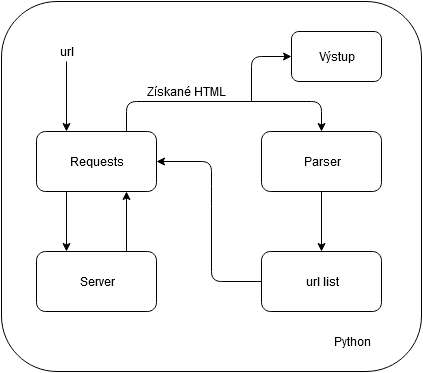
\includegraphics[width=9cm]{pictures/scrapper.png}
	\caption{Diagram zachytávání komunikace pomocí web scrapperu}
	\label{fig:web_scrapper}
\end{figure}

Obrázek \ref{fig:web_scrapper} znázorňuje cyklus získávání dat pomocí emulovaného prohlížeče. Knihovně Requests je zadána požadovaná url adresa. Knihovna získá ze serveru zdrojový kód této stránky, který uloží a zároveň jej předá html parseru. Následným výstupem je seznam url adres, které jsou ve zdrojovém kódu původní stránky obsaženy. Seznam získaných adres je nyní novým vstupem knihovny Requests. Tento cyklus se opakuje, dokud není list s url adresami prázdný. Pro cyklus je možné implementovat i hloubku procházení, aby se zabránilo nekonečné iteraci. Tento parametr určuje, do jaké úrovně se mají získávat adresy při parsování. Zde se předpokládá, že první úroveň obsahuje původní adresu, a dále každá adresa n-té úrovně je získána při parsování (n-1)-té adresy.

Nevýhodou emulace webového prohlížeče pomocí knihovny Requests je obtížná interakce se stránkami využívajícími javascript k postupnému načítání obsahu či k přesměrování na jinou adresu. Vytvořit komplexní web scrapper (tj. nástroj, který prochází obsah webových stránek), který by dokázal reagovat i na javascriptem řízený obsah, není triviální úkol.  Knihovna Requests je v tomto ohledu nedostačující a toto řešení indikuje neošetřit javascriptové přesměrování a postupné načítání obsahu.

K samotnému parsování již stažené webové stránky je možné využít knihovnu BeautifulSoup\cite{beautifulsoup}, která implementuje html a xml parsery v jazyku Python. Pomocí ní je snadné procházet html kód a iterovat přes tagy komponentů stránky. Lze tak vyhledat všechny části, které obsahují přesměrování na jiné url adresy, či spouštění javascriptového souboru. 

Přesměrování lze ošetřit pomocí hlídání response kódů (kód, který vrací server při komunikaci s webovým prohlížečem). Při přesměrování jsou běžné kódy 301, respektive 302. Pokud tedy vrátí server kód pro přesměrování, je nutné v hlavičce odpovědi najít adresu pro přesměrování a přidat ji do fronty ke zpracování.

Velkou výhodou tohoto řešení je bezpečnost, protože samotné stahování zdrojového kódu stránek probíhá bez nutnosti stažené soubory spouštět. Tímto řešením nehrozí nebezpečí infikace pracovního počítače škodlivým obsahem (o této problematice více v sekci \ref{sec:zabezpeceni}). Výraznou nevýhodou je ovšem neschopnost získání obsahu webových stránek, který se načítá asynchronně za pomoci javascriptu (využití technologie ajax).

\subsection{Zachytávání komunikace Fiddlerem}
Jiným postupem je použít nástroj Selenium(\ref{sec:selenium}) k ovládání webového prohlížeče s využitím Fiddleru(\ref{sec:fiddler}) pro zachytávání komunikace. Nevýhodou této metody je zpomalení vzniklé spouštěním internetového prohlížeče a nástroje Fiddler. Naopak výhodou je již implementované řešení webového prohlížeče umožňujícího interagovat se stránkami využívajícími javascript. Nastroj Fiddler umožňuje zachytávat i šifrovanou komunikaci pomocí protokolu https. K tomu je potřeba vygenerovat bezpečnostní certifikát a přidat jej mezi důveryhodné certifikáty v internetovém prohlížeči.

\begin{figure}[h]
	\centering
	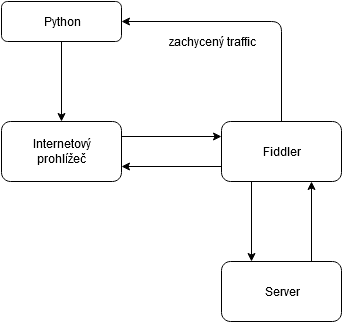
\includegraphics[width=8cm]{pictures/fiddler_diagram.png}
	\caption{Diagram zachytávání komunikace Fiddlerem}
	\label{fig:fiddler}
\end{figure}

Obrázek \ref{fig:fiddler} znázorňuje cyklus zachytávání dat pomocí nástroje Fiddler. Internetovému prohlížeči je předána adresa pomocí nástroje Selenium. Prohlížeč následně komunikuje se serverem, který vrací všechny požadované zdrojové soubory potřebné k načtení požadované adresy. Tato komunikace je zachycena pomocí nástroje Fiddler. Nástroj Fiddler je využíván k testovacím účelům a zachytává veškerou internetovou komunikaci (tzv. traffic), která skrze nástroj proudí. Využítí této metody tedy obnáší implementování třídení zachycené komunikace a selekce html a js souborů.

\subsubsection{Selekce html a js souborů}
Fiddler standardně zachytává veškerou komunikaci. Nástroj je však možné konfigurovat pomocí inicializačního scriptu, který je psaný v javascriptu. Pomocí tohoto skriptu je možné nastavit Fiddler tak, aby zachytával pouze soubory html a js. Tím lze odfiltrovat nepotřebné soubory, které se v zachycené komunikaci mohou objevit (css soubory, obrázky a jiné).

Dále je potřeba filtrovat režijní komunikaci mezi prohlížečem a servery, která vzniká při spouštění prohlížeče a načítání stránek. Tato komunikace je nevyžádaná a je potřeba ji vytřídit. I zde je možné využít inicializačního skriptu Fiddleru a implementovat třídění již při zachytávání komunikace. Zachytávat tedy pouze soubory ze serverů, které odpovídají zpracovávané url. To ovšem přináší problémy s přesměrováním, které může seznam chtěných serverů navyšovat. Druhý způsob je zachytávat html a js komunikaci ze všech serverů a selekci řešit až později při zpracování dat v Pythonu. Nedostatkem této možnosti je zvýšená náročnost na paměť při zpracovávání více souborů. Avšak předpokladem je, že tato nevyžádaná komunikace bude v poměru s chtěnými soubory minimální, tudíž by k výraznému zvýšení paměťové náročnosti dojít nemělo.





\section{Zabezpečení stahovacího procesu}\label{sec:zabezpeceni}
Z bezpečnostních důvodů je kladen důraz na zabezpečení veškerého procesu stahování webového obsahu. Při doplňování cleansetu se předpokládá neinfikovanost stažených souborů, avšak při obecnějším využití navrhovaného systému již tento předpoklad neplatí. Jedním z možných způsobů docílení bezpečnosti je vytvoření a obsluha virtuálního stroje. Tento virtuální stroj lze využít jako karanténní prostředek, který zaručí stahování souborů bez potenciální infikace fyzického systému (Obr.\ref{fig:virtualbox}).

\begin{figure}[h]
	\centering
	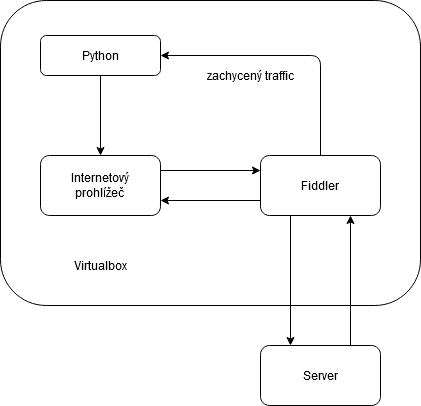
\includegraphics[width=9cm]{pictures/virtualbox.png}
	\caption{Zaobalení stahovacího procesu virtuálním strojem}
	\label{fig:virtualbox}
\end{figure}

Otevíráním webových stránek v prohlížeči dochází ke spouštění javascriptových souborů, což je potenciálně nebezpečné. Proto je zabezpečovací proces nutné řešit pouze u metody využívající nástroj Fiddler. Při emulaci prohlížeče v Pythonu dochází rovnou ke stahování zdrojových kódů webových stránek bez nutnosti jejich spouštění.

Pro virtualizaci systému lze použít nástroj VMware workstation od firmy VMware nebo VirtualBox vyvíjený firmou Oracle. Firma VMware nabízí pro práci se svými virtuálními stroji infrastrukturu nazývanou vSphere. Tato infrastruktura obsahuje vlastní SDK nástroje pro implementaci do programovacího jazyka Python\cite{vmware}, avšak celé toto řešení není nabízeno s freeware licencí. Naopak virtualizační nástroj Virtualbox(\ref{sec:virtualbox}) je zdarma, nabízí však méně propracované nástroje pro programovací jazyk Python. Pro práci s VirtualBox SDK lze využít knihovnu pyvbox\cite{pyvbox}. Tato knihova obaluje většinu metod, které SDK VirtualBoxu obsahuje. 

Virtuální stroj (neboli VM z anglického Virtual Machine) lze spouštět pro každou webovou stránku zvlášť, čímž je docíleno maximálního zabezpečení, avšak zvyšuje se tím čas potřebný ke zpracování jedné adresy. Startování VM je předpokládáno jako časově velmi náročné.  Virtuální stroj lze také restartovat vždy po určitém čase nebo po daném množství zpracovaných url adres. Tím lze docílit výrazného zrychlení běhu systému.





\section{Nahrání získaného obsahu do databáze cleansetu}
Dalším krokem je přesun získaného obsahu do samotné databáze cleansetu. Ta je součástí většího systému aplikací, který nese interní označení Scavenger. Zjednodušeně lze říci, že tento systém obsahuje záznamy o všech antiviru známých souborech a url adresách (nakažených i čistých). Soubory se v systému Scavenger indexují pomocí hashe vzniklé hashovacím algoritem sha-256. Tímto lze docílit jednoduché kontroly duplicity (stejné soubory mohou mít rozdílné názvy, ale hash souboru je pro identické soubory stejná). K hashi souboru se přikládají metadata s informací o původu souboru a času výskytu. 

K nahrání souborů do Scavengeru lze využít síťový souborový systém Samba, který implementuje přenos souborů po síti pomocí síťového protokolu SMB a to převážně v systémech Windows. Tato metoda je však z hlediska firemní infrastruktury zastaralá. Novější způsob představuje využití datové platformy HCP (Hitachi content platform) \cite{hcp}. Tato platforma se specializuje na přesun a zpracování velkého množství dat z různých zdrojů. Ke komunikaci se zmíněným systémem HCP lze využít interně vyvinutý python klient, který přesun souborů usnadní.





\section{Začlenění do stávající infrastruktury}
Předpokládá se, že systém bude spouštěn periodicky, ale měl by být také spustitelný na vyžádání uživatelem. Pro takové požadavky lze použít systém Jenkins(\ref{sec:jenkins}), který je firmou Avast používaný ke správě obdobných aplikací. Jednotlivé části aplikace Magpie je možné rozdělit do samostatných procesů (v terminologii systému Jenkins tzv. jobů), které se dají sekvenčně pouštět v závislosti na úspěšném ukončení předcházejícího jobu. Tento přístup přináší přehledné rozhraní, které umožňuje jednotlivé části samostatně monitorovat, spolu s jednoduchým přístupem k výstupům jobů. Tímto způsobem by bylo možné přistoupit k získaným datům přímo, bez nutnosti data nahrávat do databáze v systému Scavenger, v případě, kdy by byl systém spuštěný manuálně.

Jiným přístupem je využít firemní mutaci nástroje Kubernetes, která by umožňovala mít systém spuštěný bez přestávky. Krom neustálého spuštění skriptu je velkou výhodou Kubernetes tzv. škálování, kdy lze při velkém vytížení jednoduše navýšit výpočetní prostředky danému procesu a tím urychlit jeho běh. Pro spuštění skriptu v Kubernetes je nejprve potřeba tento skript dockerizovat. Dockerizace je proces, při kterém je vytvořen tzv. docker image, neboli balíček, který je plně spustitelný ve virtualizovaném prostředí, například v Kubernetes. Při dockerizaci je nutné vytvořit \mintinline{Python}{Makefile}, který obsahuje informace o vzniku balíčku. 

Je také možné pro jednotlivé části systému Magpie využít rozdílné technologie, například kombinaci obou výše zmíněných.

\section{Programovací jazyk}
Převážná část práce bude psána v programovacím jazyku Python\cite{python}. Python obsahuje velké množství dostupných knihoven, čímž lze docílit snadné integrity mezi jednotlivými komponentami aplikace Magpie. Tato volba je i v souladu s firemní politikou. 

Při volbě stahování dat s využitím nástroje Fiddler bude dalším využitým programovacím jazykem JavaScript, neboť v tomto jazyku je psán inicializační soubor zmíněného nástroje.
















\chapter{Použité technologie}
V této kapitole jsou stručně popsány všechny technologie využité při zpracovávání této práce.

\section{Python}\label{sec:python}
Python je skriptovací programovací jazyk, jehož syntaxe je lehce odlišná od konvenčních programovacích jazyků (Java, C). Jedná se o hybridní programovací jazyk, což znamená, že program nemusí být nutně objektově orientovaný, ale části mohou mít více procedurální charakter. Tím dochází k lepší čitelnosti kódu a celkovému zjednodušení. Síla Pythonu je i ve velkém množství balíků s knihovnami, které podporují jeho všestrannost. Zároveň je tento programovací jazyk velmi rozšířený ve firmě Avast. Kvůli těmto okolnostem byl vybrán Python 3.7 jako hlavní programovací jazyk pro tuto diplomovou práci.

\section{Fiddler}\label{sec:fiddler}
Fiddler\cite{fiddler} je nástroj vyvíjen firmou Telerik, sloužící k zachytávání internetové komunikace. Funguje na principu MitM (Man-in-the-middle) útoku, kdy se prostředník vtěsná mezi dva účastníky internetového provozu a nechá je komunikovat skrz sebe (Obr.\ref{fig:mitm}).
\begin{figure}[h]
	\centering
	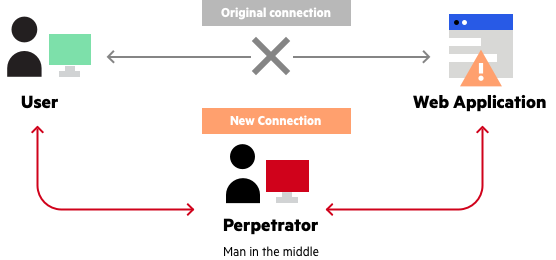
\includegraphics[width=9cm]{pictures/mitm.png}
	\caption{MitM útok \cite{mitm}}
	\label{fig:mitm}
\end{figure}
Fiddler může být automatizován pomocí inicializačního souboru, který obsahuje různá pravidla a je psaný v javascriptu. Při správném nastavení je Fiddler schopný zachytávat i šifrovanou komunikaci.

\section{Selenium} \label{sec:selenium}
Selenium je opensource nástroj používaný k automatizovanému přístupu k webovým aplikacím. Těchto vlastností se často využívá při testování, avšak v této práci je použit pouze k obsluze webového prohlížeče. Selenium obsahuje vlastní vývojové prostředí, které lze využít bez velké znalosti programování, existují však i jeho implementace do většiny populárních programovacích jazyků. V této práci je využita knihovna Selenium pro programovací jazyk Python.


\section{Jenkins} \label{sec:jenkins}
Jenkins je opensource CI/CD systém (continuous integration/continuous delivery) umožňující vykonávání automatických či periodických operací (tzv. jobů) a používá se převážně ke spouštění skriptů. Joby lze spoustět různými způsoby. Pravidelně v předem určený čas, na vyžádání přes webové rozhraní, pomocí api, či automaticky po doběhnutí jiného jobu.

\section{Kafka}\label{sec:kafka}
Kafku lze řadit mezi frontové systémy. Jedná se o opensource platformu sloužící ke streamování dat v reálném čase. Její zaměření je převážně na zpracování velkého množství zpráv bez narůstající latence. Zprávy se však neukládají do fronty, jako je tomu u některých jiných frontových systémů, např. RabbitMQ, avšak do tzv. topiců. Jeden topic může obsahovat více částí (tzv. partition), do kterých se zprávy distribuují (Obr.\ref{fig:kafka}). 
\begin{figure}[h]
	\centering
	
\includegraphics[width=9cm]{pictures/kafka.png}
	\caption{Znázornění Kafka systému \cite{kafka}}
	\label{fig:kafka}
\end{figure}
Zprávy do topicu posílá proces, který se nazývá producer. Obdobně proces, který data čte, je nazýván consumer. Ten dostává zprávy z topicu v závislosti na indexaci a časové známky. K jednomu topicu může být přihlášeno více nezávislých consumerů, které jsou rozděleny do odlišných skupin (tzv. Group ID) a každá skupina dostává identické zprávy. Tím je zabráněno vzájemnému čtení stejných zpráv.

Tato politika čtení zpráv je velkou výhodou oproti zmiňovanému systému RabbitMQ, kde po přečtení zpráva mizí. 

Zprávy zůstávají v topicu po určitou dobu, kterou určuje hodnota retence. Po tuto dobu jsou zprávy přístupny pro každou skupinu consumerů. V Kafce funguje tzv. potvrzovací systém. Consumer dostane zprávu, a po jejím zpracování vyšle tzv. commit, kterým oznámí úspěšné zpracování. Pokud by v průběhu nastala chyba, tento commit se nepošle a zpráva se vrátí zpátky, kde může být přečtena jiným consumerem ve skupině.

\section{VirtualBox}\label{sec:virtualbox}
VirtualBox je opensource virtualizační nástroj vyvíjený firmou Oracle. Slouží k instalaci  a obsluze virtuálních operačních systémů na jednom fyzickém stroji. Jeho výhodou je multiplatformnost, což znamená, že je možné ho nainstalovat na MS Windows i operační systémy s unixovým jádrem (Linux, Mac OS). Tímto lze docílit například spuštění linuxového systému pod operačním systémem Windows.\cite{virutalbox}
\begin{figure}[h]
	\centering
	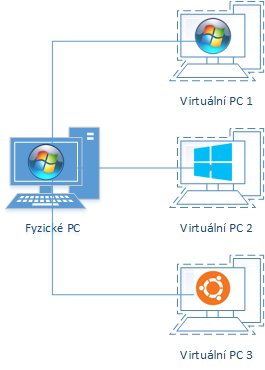
\includegraphics[width=7cm]{pictures/vbox.png}
	\caption{PC s virtuálními stroji \cite{vbox_pic}}
	\label{fig:vbox}
\end{figure}

Další důležitou funkcionalitou VirtualBoxu jsou tzv. snapshoty. Snapshot zachycuje virtuální stroj a veškeré jeho nastavení v daném čase, ve kterém je vytvořen. Tímto lze jednoduše vracet provedené změny zpět do bodu vytvoření snapshotu. Toho je možné využít při testování aplikací, využití je avšak možné i v oblasti bezpečnosti. Pokud je vytvořen snapshot čistého systému, lze se do něj vrátit v případě potenciálního nakažení virtuálního stroje.


\section{Docker}\label{sec:docker}
Docker je souhrn produktů typu PaaS (platform as a service) vyvíjený firmou Docker, Inc. \cite{docker}. Služba využívá virtualizaci operačních systémů či jiných platforem k vytvoření tzv. kontejnerů. Tyto kontejnery obsahují vlastní knihovny a konfigurace, ke spuštění však potřebují centrální systém nazývaný Docker Engine. V tomto je tato služba oproti virtuálním strojům (např. Virtualbox) více odlehčená, nevýhodou je však nutnost centrálního operačního systému. 

\begin{figure}[H]
	\centering
	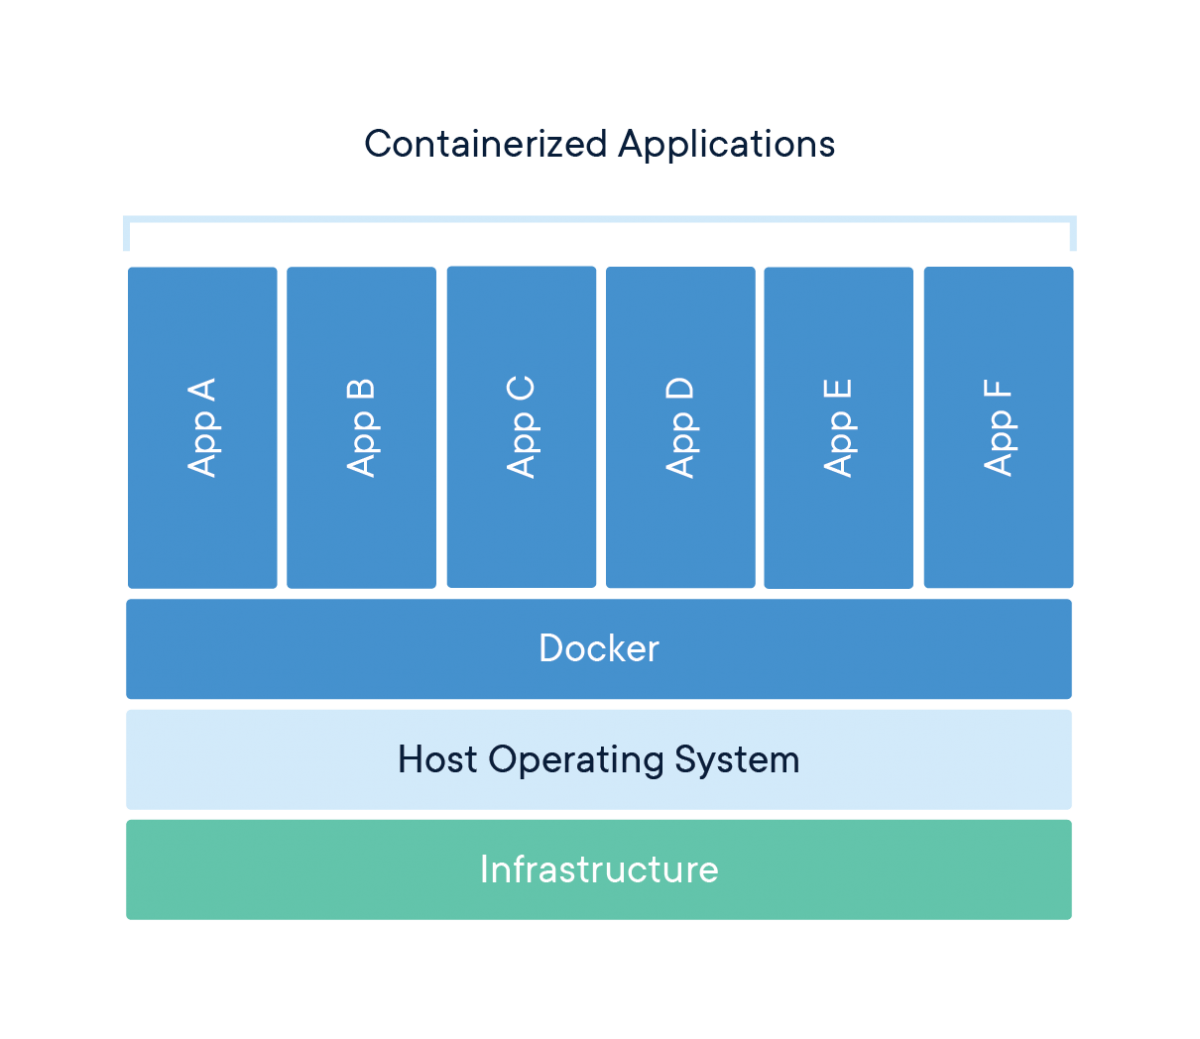
\includegraphics[width=10cm]{pictures/docker.png}
	\caption{Systém s dockerizovanými aplikacemi \cite{docker}}
	\label{fig:docker}
\end{figure}



K dockerizaci aplikace je potřeba vytvořit tzv. Dockerfile, který obsahuje sekvenci příkazů k sestavení kontejneru. Ten je poté možné spustit ve službě Kubernetes dostupné firmou Docker, Inc. Tato služba je tzv. Task Manager, neboli systém, v kterém je možné spravovat jednotlivé procesy, zde spuštěné instance kontejnerů.













\chapter{Implementace}
Z analýzy je patrné, že by zvoleným programovacím jazykem pro systém Magpie měl být Python. Prvním krokem implementace projektu je vytvořit funkční jádro, ke kterému by bylo možné přidávat ostatní komponenty a vylepšovat jeho funkcionalitu. Za toto jádro lze považovat stahování zdrojového kódu stránek. Následně je potřeba tento proces zabezpečit, zdokonalit a integrovat do stávající infrastruktury Avastu. Jednotlivé sekce implementace jsou následující:
\begin{itemize}
	\item Klient pro stahování webového obsahu
	\item Zpracování dat a upload do databáze
	\item Virtualizace 
	\item Implementace frontového systému Kafka
	\item Integrace pomocí systému Jenkins
\end{itemize} 




\section{Klient pro stahování webového obsahu} \label{sec:stahovani}
Při implementaci klientu pro stahování webového obsahu byla zvolena metoda s využitím programu Fiddler pro zachytávání internetové komunikace. Tato metoda přináší komplexnější odposlech bez nutnosti emulace webového prohlížeče. Bylo nutné vytvořit skript pro ovládání internetového prohlížeče a Fiddleru, tento skript byl napsaný v jazyku Python, a dále bylo zapotřebí nastavit Fiddler pomocí inicializačního souboru, který je napsaný v javascriptu. Sekce je tedy rozdělena do dvou podsekcí:
\begin{itemize}
	\item Skript pro ovládání pomocných programů
	\item Skript pro nastavení Fiddleru
\end{itemize}

\subsection{Skript pro ovládání pomocných programů}
Tento skript je psaný v programovacím jazyku Python, stejně jako většina práce. Jeho hlavní činností je spuštění programu Fiddler a správa internetového prohlížeče. K ovládání webového prohlížeče byl použit nástroj Selenium(\ref{sec:selenium}) v podobě knihovny importované do jazyka Python. Pro komunikaci s webovým prohlížečem je nutné nainstalovat takzvaný webdriver, který zajistí správnou konfiguraci Selenia pro daný prohlížeč. Webdriver Geckodriver\cite{gecko} je určený pro komunikaci s internetovým prohlížečem Mozilla Firefox\cite{firefox}, naproti tomu webdriver ChromeDriver\cite{chromedriver}  je vyvinut  pro komunikaci s internetovým prohlížečem Google Chrome\cite{chrome}. V práci byl využit internetový prohlížeč Mozilla Firefox, tudíž i nástroj Geckodriver.

Základní implementace Selenia s ovládáním webového prohlížeče v jazyku Python může vypadat jako ve výřezu kódu (tzv. snippetu) \ref{snip:selenium}.

\begin{figure}[h]               
\begin{minted}{Python}
import time

from selenium.webdriver import Firefox
from selenium.webdriver.firefox.options import Options

opts = Options()
opts.headless = True

browser = Firefox(options=opts)
browser.get("https://www.seznam.cz")

time.sleep(2)
browser.quit()
\end{minted}      
\caption{Implementace nástroje Selenium s ovládáním prohlížeče}
\label{snip:selenium}
\end{figure}
Selenium nabízí možnost konfigurace webdriveru, což umožnuje nastavovat různé parametry. V tomto případě je zvolen přepínač \mintinline{Python}{headless}, který určuje spouštění webového prohlížeče bez grafického uživatelského prostředí (tzv. GUI), čímž lze docílit rychlejšího průběhu. Samotné načtení webové stránky se provádí pomocí metody \mintinline{Python}{get()}, která přijímá v parametru url stránky (ve snippetu stránka \mintinline{Python}{https://www.seznam.cz}). Příkazem \mintinline{Python}{quit()} lze internetový prohlížeč zavřít. Metoda \mintinline{Python}{get()} je implementována, aby čekala na úplné načtení stránky, avšak nepočítá s asynchronním načítáním. Pro kompletní načtení webové stránky je tedy potřeba přidat časovač (tzv. timer), který před zavřením prohlížeče skript pozastaví na určitou dobu (zde 2 sekundy).




\subsection{Skript pro nastavení Fiddleru}\label{sec:fiddler_setup}
Program Fiddler se primárně ovládá přes grafické rozhranní, je však možné změnit jeho výchozí konfiguraci. K tomuto účelu slouží inicializační skript, který nese označení \mintinline{Python}{CustomRules.js}, jedná se tedy o skript psaný v javaScriptu. Fiddler při spuštění vždy načítá set pravidel, podle kterých se nastaví. Defaultně jsou tato pravidla brána ze skriptu, který se nachází v instalačním adresáři programu. Skriptem \mintinline{Python}{CustomRules.js} lze tyto pravidla nahradit.

\begin{figure}[h]               
	\begin{minted}{Javascript}
static function OnBeforeResponse(oSession: Session) {
	
  var code = oSession.responseCode
  if (code == 200 || code == 301 || code == 302) {
	
    var path = "c:\\tmp\\fiddler_data\\"
    var filename_dat  = path + oSession.id + ".dat";
    var filename_meta = path + oSession.id + ".meta";
	
    System.IO.File.WriteAllBytes(
    filename_dat, oSession.responseBodyBytes);
	
    var url = oSession.url;
    var host = oSession.host);
    var referer = oSession.oRequest.headers["Referer"]);
    var response = oSession.responseCode);
    var redirect = oSession.oResponse.headers["Location"]);
    var time = System.DateTime.Now);
	
    WriteMeta(url, host, referer, response, redirect, time)
  }
}
	\end{minted}      
	\caption{Implementace inicializačního skriptu Fiddleru}
	\label{snip:fiddler}
\end{figure}

Skript obsahuje mnoho funkcí pro různé sekce programu, z hlediska této práce je však důležitá pouze funkce \mintinline{Python}{OnBeforeResponse()}, která je zavolána vždy, když přijde ze serverové části nějaká odpověď (tzv. response). Implementace této metody je znázorněna v snippetu \ref{snip:fiddler}.

Tělo funkce \mintinline{Python}{OnBeforeRequest()} obsahuje jedinou podmínku založenou na kódu odpovědi (tzv. response kód) serverové části. Tento kód se nejdříve získá z relace oSession (relace, která obsahuje veškeré informace o komunikaci s danou url). Pokud je response kód $200$, jedná se o tzv. \mintinline{Python}{success} (úspěch), což znamená, že server na daný dotaz prohlížeče vrací odpověď. Tento typ odpovědí je snaha zachytávat, neboť obsahují zdrojové soubory webových stránek. Pokud se však stránka na serveru nachází jinde než na prohlížečem dotazované url, může dojít k přesměrování. Response kódy pro přesměrování zpravidla spadají do intervalu $300-399$, avšak nejčastější případy přesměrování mají kódy $301$, respektive $302$. Kód $301$ je rezervován pro trvalá přesměrování (tzv. moved permanently), kód $302$ dříve sloužil pro přesměrování dočasná (tzv. moved temporarily), od standardu HTTP/1.1 je však více využíván pro všeobecná přesměrování\cite{response_codes}. Pokud tedy dojde k zachycení odpovědi, která obsahuje jeden z těchto tří kódů, podmínka je splněna.

Při nastání této situace jsou vytvořeny dva soubory, které jsou pojmenovány podle id relace. Soubor s koncovkou \mintinline{Python}{.dat} je určený pro záznam zachycených dat, soubor \mintinline{Python}{.meta} slouží k uchování metadat o zachycené komunikaci. Následně se volá funkce \mintinline{Python}{WriteAllBytes()}, která z relace oSession přijme parametr \mintinline{Python}{responseBodyBytes}, který obsahuje tělo odpovědi ze serveru, tedy zachycená data, a zapíše je do datového souboru. Dále se shromáždí metadata potřebná pro filtraci souborů (Tabulka \ref{fig:meta}), která se zapíší do souboru \mintinline{Python}{.meta}. 


\begin{table}[h]
	
	\centering
	\begin{tabular}{ll}
		url         	&  zdrojová stránka souboru \\
		host        	&  název serveru, na kterém je zdrojová stránka \\
		referer       	&  stránka, z které přišla žádost o načtení současné url \\
		response kód   	&  kód, který byl zaznamenán v hlavičce souboru  \\
		redirect		&  destinace v případě přesměrování \\
		time			&  čas záznamu souboru
	\end{tabular}
	
	\caption{Metadata stažených souborů}
	\label{fig:meta}
\end{table}



\section{Zpracování dat a upload do databáze}
Protože byl ke stahování dat použit program Fiddler, který zaznamenává kompletní komunikaci prohlížeče s webovým serverem, je potřeba stažená data profiltrovat. K tomuto účelu byl vytvořen skript v programovacím jazyku Python. Následně je zapotřebí protříděná data nahrát do systému Scavenger, kde se nachází databáze cleansetu. Tato sekce tedy může být rozdělena na dvě části:
\begin{itemize}
	\item Třídění dat
	\item Upload do databáze
\end{itemize}



\subsection{Třídění dat}\label{sec:trideni}
Pro potřeby třídení dat byl program Fiddler konfigurován, aby spolu se zdrojovým kódem webových stránek zaznamenával i pomocná metadata. Tato metadata jsou využívána v Python skriptu, který třídění dat implementuje. Vstupem skriptu je setříděný list, který obsahuje stažená data, spolu s jejich metadaty. Tyto soubory jsou inkrementálně očíslovány podle toho, v jakém pořadí byly Fiddlerem zaznamenány (implementováno v inicializačním skriptu Fiddleru \ref{sec:fiddler_setup}).

Protože Fiddler zaznamenává veškerou komunikaci, je zapotřebí odlišit komunikaci vyvolanou přístupem na požadovanou webovou stránku od zbylé (např. režijní komunikace mezi prohlížečem a serverem). První soubor, který je v sekvenčním průchodu důležitý, bude v metadatech obsahovat požadovanou webovou stránku v hodnotě pole \textit{url} (viz tabulka s metadaty \ref{fig:meta}). Hlavní smyčka třídícího skriptu je znázorněna na snippetu \ref{snip:filter}. 

\begin{figure}[h]               
\begin{minted}{Python}
sorted_list = get_files_ids(directory)
stripped_url = netloc_from_url(url)
referers = {stripped_url}
valid_ids = []

for file_id in sorted_list:
    data = f"{directory}/{file_id}.dat"
    meta = get_meta_from_file(f"{directory}/{file_id}.meta")

    netloc_url = netloc_from_url(meta["url"])
    netloc_referer = netloc_from_url(meta["referer"])
    netloc_redirect = netloc_from_url(meta["redirect"])

    response = meta["response_code"]
    redirect_response = response == 301 or response == 302
    
    if redirect_response and meta["host"] in referers:
        if meta["redirect"] is not "":
            referers.add(netloc_redirect)
    elif os.path.getsize(data) < 9:
        continue
    elif netloc_url in referers or (
        netloc_referer is not "" and 
        netloc_referer in referers
    ):
        valid_ids.append(file_id)
        referers.add(netloc_url)

\end{minted}      
\caption{Implementace filtrování stažených dat}
\label{snip:filter}
\end{figure}

Metoda \mintinline{Python}{get_file_ids()} načítá id stažených souborů (očíslováno podle zaznamenaného pořadí) a ukládá je do listu, přes který iteruje hlavní smyčka skriptu. Metoda \mintinline{Python}{netloc_from_url()} vrací netloc (tj. doménové jméno první úrovně) zadané adresy. Každá url adresa se řídí daným formátem, zjednodušeně takto:
\begin{eqnarray}
<scheme>://<netloc>/<path>
\end{eqnarray}
Pro příklad \url{http://www.example.com/index} je tedy \mintinline{Python}{http} schéma, \mintinline{Python}{index} cesta a \mintinline{Python}{www.example.com} hledaný netloc. Toho bylo použito při procházení setříděného listu očíslovaných souborů. Před iterací je ještě zapotřebí inicializovat dvě datové struktury. Set \mintinline{Python}{referers} bude obsahovat všechny již známé a chtěné referery (tj. netloc adresy, které si vyžádaly načtení zdrojových souborů současné url \ref{fig:meta}). Jak již bylo dříve zmíněno, prvním takovým refererem je původní zadaná adresa. Druhá struktura, list \mintinline{Python}{valid_ids}, bude uchovávat názvy souborů, které byly vyhodnoceny jako validní (tj. soubory zachycené při komunikaci s původní zadanou adresou).

V hlavní smyčce se nejprve načtou metadata k souboru pomocí metody \mintinline{Python}{get_meta_from_file()} a uloží se do slovníku \mintinline{Python}{meta}. Poté se tyto data oříznou pomocí metody \mintinline{Python}{netloc_from_url()} a dále se pracuje jen s jejich netloc částí. První podmínka vyhodnocuje přesměrování. Pokud je \mintinline{Python}{response_code} v metadatech souboru roven $301$ nebo $302$, což značí přesměrování, a pokud je zároveň \mintinline{Python}{host} této adresy již v setu \mintinline{Python}{referers}, nejedná se o validní soubor, jde však o soubor, který nese informace o přesměrování. Je tedy potřeba přidat netloc adresy, na kterou dojde k přesměrování (v metadatech klíčové slovo \mintinline{Python}{redirect}). 

Druhá podmínka je přidána pro optimalizaci. Fiddler zaznamenává velké množství souborů, které mají režijní charakter. Tyto soubory se vyznačují malou velikostí a jsou z hlediska filtrace nedůležité. Z toho důvodu se dál zpracovávají pouze soubory, které mají více než 8 bytů.

Poslední podmínka již kontroluje samotné validní soubory. Pokud je netloc adresy nebo netloc referera adresy již v setu \mintinline{Python}{referers}, jedná se o soubor zachycený při komunikaci s cílovou adresou a soubor je přidán do validního listu. Dále je netloc adresy přidán do \mintinline{Python}{referers} z důvodu, kdy by tato adresa odkazovala na jinou url při další komunikaci. Po iteraci nad všemi soubory v setříděném listu je výstupní list \mintinline{Python}{valid_ids} předán ke zpracování skriptu pro upload dat do databáze.





\subsection{Upload do databáze} \label{sec:upload}
Pro nahrávání dat do databáze byl již dříve týmem, který spravuje systém Scavenger, vytvořen klient v podobě python knihovny. Tento klient používá HCP (Hitachi content platform) pro přesun dat mezi klientem a servery Scavengeru a představuje novější řešení oproti dříve používanému klientu Samba. Při uploadu dat do databáze lze tedy vycházet z tohoto kódu. V prvním kroku procesu uploadu do Scavengeru klient přesune požadovaný soubor do tzv. namespace (vyhrazený prostor na serverové části unikátní pro daného klienta) v HCP úložišti a připojí k němu požadovaná metadata. K tomuto namespace je připojen proces (tzv. feeder), který periodicky odebírá přítomné soubory i s jejich metadaty a přesouvá je do systému Scavenger, kde jsou soubory indexovány pomocí hashovací funkce sha256.

Implementace klientu je velmi jednoduchá (snippet \ref{snip:hcpupload}).
\begin{figure}[h]               
	\begin{minted}{Python}
def upload_file(file, target_name, meta):
    client = Client(**config.HCP_CONFIG)
    client.upload_object(file, target_name, meta)
	\end{minted}      
	\caption{Implementace použití HCP klientu pro upload}
	\label{snip:hcpupload}
\end{figure}
Z knihovny je potřeba provést import třídy \mintinline{Python}{Client()} a její inicializaci, při které se předává konfigurace klientu. Konfigurace obsahuje jméno \mintinline{Python}{namespace}, tedy cílový prostor v úložišti, ke kterému se připojit, přihlašovací jméno a heslo. Všechny tyto údaje byly vygenerovány týmem spravující HCP úložiště. Dále už stačí jen volat metodu \mintinline{Python}{upload_object()} a předat jí potřebné parametry. Mezi tyto parametry paří cesta k nahrávanému souboru (\mintinline{Python}{file}), název, jaký ponese soubor v úložišti (\mintinline{Python}{target_name}), a požadovaná metadata, která se mají k souboru přiložit (\mintinline{Python}{meta}). Zde není potřeba nahrávat všechna metadata získaná při stahování souborů. Ve snippetu \ref{snip:metaupload} je kód, který tento výběr zajišťuje.

\begin{figure}[h]               
	\begin{minted}{Python}
def set_meta_for_upload(meta_file, url):
    meta = {
        "source_url": meta_file["url"],
        "source_url_referer": meta_file["referer"],
        "trigger_url": url,
    }
	
    return meta
	\end{minted}      
	\caption{Implementace načtení metadat pro HCP upload}
	\label{snip:metaupload}
\end{figure}

Metoda \mintinline{Python}{set_meta_fot_upload()} má dva vstupní parametry. Prvním je slovník \mintinline{Python}{meta_file}, který obsahuje všechna stažená metadata, druhým je \mintinline{Python}{url}, což je původní dotazovaná adresa. Výstupem metody je slovník s metadaty určenými pro upload do HCP úložiště. Pro soubor uložený na cleansetu je důležitý údaj o adrese, na které se soubor vyskytoval – \mintinline{Python}{source_url} – a kdo na tuto adresu odkazoval – \mintinline{Python}{source_url_referer}. Třetím důležitým údajem je původní volaná adresa \mintinline{Python}{trigger_url}. Ta je důležitá v případě, že by se na cleansetu objevily dva totožné soubory. V takové situaci se nový soubor již nepřidá, aktualizují se však jeho metadata a v budoucnu je stále patrné, že byl tento soubor viděn při komunikaci s vícero rozdílnými adresami.

\begin{figure}[h]               
	\begin{minted}{Python}
for counter, file in enumerate(filenames):
    file_name = f"{root}\\{directory}\\{file}"
	
    meta = hcp_feeder.set_meta_for_upload(
        files_filter.get_meta_from_file(f"{file_name}.meta"),
        directory
    )
	
    hcp_feeder.upload_file(
        f"{file_name}.dat",
        f"{directory}{counter}",
        meta
    )
	\end{minted}      
	\caption{Implementace hlavní smyčky pro upload}
	\label{snip:mainupload}
\end{figure}

Snippet \ref{snip:mainupload} znázorňuje hlavní smyčku skriptu pro upload souborů do HCP úložiště a následně do Scavengeru. V ní dochází k iteraci přes všechny validní soubory (výstup z třídění dat \ref{sec:trideni}). Pro každý soubor se nejdříve určí cesta souboru \mintinline{Python}{file_name}. Následně se nastaví metadata pro upload zavoláním metody \mintinline{Python}{set_meta_for_upload()}, které se předá cesta k souboru s metadaty a původní tázaná url (zde \mintinline{Python}{directory} z důvodu, že se stažené soubory ukládají do složek pojmenovaných podle původní zadané adresy). Na závěr cyklu hlavní smyčky je volána funkce \mintinline{Python}{upload_file}. Prvním parametrem je cesta k datovému souboru. Následuje cílový název souboru v HCP úložišti. Zde, aby se zajistila unikátnost souborů v úložišti, se soubory přejmenovávají podle klíče:
\begin{center}\label{prejmenovavani}
\{původní\_ adresa\}\{pořadí\_ zpracovaného\_ souboru\}
\end{center}

 Toto je možné z důvodu, že se následně soubory automaticky přejmenovávají při přenosu z HCP úložiště do Scavengeru pomocí hashovací funkce sha256. Posledním parametrem pro upload jsou metadata souboru.

\section{Virtualizace}
Z důvodu použití programu Fiddler pro stahování dat namísto emulace webového prohlížeče v Pythonu je nutné tento proces zabezpečit (výsledek analýzy v sekci \ref{sec:zabezpeceni}). Toho bylo docíleno obalením stahovacího procesu do virtuálního prostředí díky využití programu Virtualbox. K tomu byla využita knihovna \mintinline{Python}{pyvbox}\cite{pyvbox}, která implementuje Virtualbox API v prostředí Pythonu. Není potřeba virtualizovat celý proces, ale jen část, která se zabývá stahováním dat. Bylo tedy zapotřebí vytvořit skript, který dokáže nastartovat virtuální stroj, v něm spustit aplikaci pro stahování souborů a tyto soubory přenést z virtuálního prostředí zpět do fyzického systému.

K tomuto účelu byla vytvořena třída  \mintinline{Python}{Vbox}, jejíž inicializace (tzv. konstruktor) je zobrazena ve snippetu \ref{snip:vboxmain}. Instanci této třídy lze použít k ovládání virtuálního stroje. K tomu je nutné inicializovat tři objekty – \mintinline{Python}{VirtualBox()}, \mintinline{Python}{Session()} a \mintinline{Python}{Machine()}. Instance třídy \mintinline{Python}{VirtualBox()} slouží k ovládání Virtualbox manažeru (program, který řídí jednotlivé zaregistrované virtuální stroje). Obecné nastavování se tedy provádí přes tento objekt. Třída \mintinline{Python}{Session()} je navázána na relaci konkrétního virtuálního stroje. Ovládání běhu stroje probíhá tedy s využitím tohoto objektu. Třída \mintinline{Python}{Machine()} reprezentuje konkrétní stroj tak, jak je zobrazen v manažeru Virtualboxu. Při inicializaci této třídy je zapotřebí předat název stroje, což je zde řešeno pomocí převzaté metody \mintinline{Python}{find_machine()}. Název stroje je možné předat konstruktoru pomocí parametru \mintinline{Python}{machine}. Pokud není žádný konkrétní stroj vybrán, je proveden výčet všech dostupných strojů přihlášených pod Virtualbox manažerem (metoda \mintinline{Python}{list_all_machines}) a načten první dostupný stroj.
\begin{figure}[h]               
	\begin{minted}{Python}
import virtualbox

class Vbox:
    def __init__(self, machine=""):

    # init virtualbox
    self.vbox = virtualbox.VirtualBox()

    # init session
    self.session = virtualbox.Session()

    # define machine and create a session
    machines = self.list_all_machines(self.vbox)
    if machine not in machines:
        if len(machines) == 0:
            print("No virtual machines to load")
            sys.exit()

        print(
            "No or corrupted machine name, "
            f"loading machine {machines[0]}"
        )
        machine = machines[0]

    self.machine = self.vbox.find_machine(machine)
	\end{minted}      
	\caption{Implementace inicializace třídy Vbox}
	\label{snip:vboxmain}
\end{figure}


Pro ovládání spuštění virtuálního stroje s časováním byla vytvořena metoda \mintinline{Python}{boot_with_timeout()} (snippet \ref{snip:vboxboot}). Tato metoda přijímá tři parametry. Prvním parametrem je \mintinline{Python}{timeout}, neboli čas, po kterém se metoda přeruší a zabrání se tak případnému nekonečného cyklu. Další dva parametry jsou přihlašovací jméno a heslo do uživatelského účtu ve virtuálním systému. Tyto údaje jsou potřeba pro inicializaci uživatele, ke které v průběhu spouštění systému (tzv. bootování) dochází. Na začátku je zavolána metoda \mintinline{Python}{launch_machine()}, která zahájí proces bootování. Aby nedocházelo k nepředvídatelnému průběhu, volá se zde další metoda \mintinline{Python}{wait_for_session_locked()}, která zajišťuje, že bootovací proces nebude pokračovat, dokud se neuzamkne virtuální stroj (parametr \mintinline{Python}{machine} třídy \mintinline{Python}{Vbox}) pro současnou relaci (parametr \mintinline{Python}{session}). Při ovládání stroje skrze neuzamčenou relaci může nastat chyba a následné ukončení skriptu. 
\begin{figure}[h]               
	\begin{minted}{Python}
def boot_with_timeout(self, timeout, login, password):

    self.launch_machine()
    self.wait_for_session_locked()

    t_boot = 1

    while t_boot < timeout:

        print(f"Booting... ({t_boot}/{timeout})")
        try:
            gs = self.login(login, password)
            gs.directory_exists("c:/")
            print("Machine has started.")
            return gs

        except virtualbox.library.VBoxError as e:
            print(f"Machine not started yet: {e}")

        time.sleep(1)
        t_boot += 1

    raise DidntBootInTimeException(
        "Timeout reached. Machine didn't boot in time."
    )
	\end{minted}      
	\caption{Implementace bootovacího algoritmu pro VirtualBox}
	\label{snip:vboxboot}
\end{figure}


Poněvadž VirtualBox API nemá implementovanou kontrolu průběhu bootování, nelze nijak zkontrolovat, zda je už virtuální stroj načtený a připravený k použití. Z tohoto důvodu je vytvořen \textit{while} cyklus, kde k této kontrole periodicky dochází. V každém průběhu cyklu dochází k inicializaci uživatelského účtu a následnému testu existence kořenové složky c:/ metodou \mintinline{Python}{directory_exists()}. Předpokládá se zde, že dojde k chybě, protože systém ještě není připravený takovéto příkazy zpracovávat. V takové situaci je výjimka odchycena a přechází se na další průběh cyklu. Pokud by již metoda \mintinline{Python}{directory_exists()} proběhla bez chybové hlášky, dá se očekávat, že je systém již připravený k používání. V tomto případě dojde k ukončení metody. Výstupem je objekt s inicializovaným uživatelským účtem v případě, že bootování proběhlo bez problémů, či chybová hláška \mintinline{Python}{DidntBootInTimeException} v situaci, kdy vypršel časový limit dříve, než mohl systém naběhnout.

\begin{figure}[h]               
	\begin{minted}{Python}
commands = (
    f"cd c:/tmp & "
    f"python {config.VBOX_SCRIPT_PATH} {url}"
)
gs.execute(
    "C:\\Windows\\System32\\cmd.exe", 
    ["/C", commands]
)
	\end{minted}      
	\caption{Spouštění příkazů ve virtuálním systému}
	\label{snip:vboxcommand}
\end{figure}
S již vytvořeným objektem uživatelského účtu lze následně spouštět příkazy přes příkazový řádek (tzv. command line) virtuálního systému (snippet \ref{snip:vboxcommand}), kde parametr \mintinline{Python}{commands} obsahuje jednotlivé příkazy, tedy přesun do pracovní složky a spuštění skriptu pro stahování webového obsahu (viz sekce \ref{sec:stahovani}) s parametrem požadované adresy url.

Pro přesun stažených souborů z virtuálního prostředí do reálného systému byla převzata metoda \mintinline{Python}{directory_copy_from_guest()} (snippet \ref{snip:vboxcopy}),
\begin{figure}[h]               
	\begin{minted}{Python}
gs.directory_copy_from_guest(
    dir_from_path,
    dir_to_path,
    [virtualbox.library.DirectoryCopyFlag(1)]
)
	\end{minted}      
	\caption{Spouštění příkazů ve virtuálním systému}
	\label{snip:vboxcopy}
\end{figure}
 která je implementována ve třídě pro uživatelský účet virtuálního stroje. Tato metoda kopíruje celou složku, která je předána v parametru \mintinline{Python}{dir_from_path}, do cílové lokace specifikované paramterem \mintinline{Python}{dir_to_path}. Třetím parametrem metody je konfigurační hodnota (tzv. flag), která určuje typ přenosu.








\section{Implementace frontového systému Kafka}

Dalším krokem je implementace frontového systému Kafka, jehož serverová část je součástí firemní infrastruktury. K těmto účelům byly vygenerovány týmem spravujícím interní mutaci Kafky přihlašovací údaje pro systém Magpie (přihlašovací jméno, heslo a SSL certifikát). Pro implementaci samotného klientu byla použita Python knihovna \mintinline{Python}{confluent-kafka}\cite{confluent-kafka}, jejíž výhodou je možnost zabezpečené komunikace klientu se serverem. Byly vytvořeny dva skripty obsahující rozdílné klienty:
\begin{itemize}
	\item Kafka producer
	\item Kafka consumer
\end{itemize}


\subsection{Kafka producer} \label{sec:kafkaproducer}
Úkolem skriptu implementujícího klienta Kafka producer je posílání předzpracovaných url do frontového systému. Za tímto účelem byla vytvořena třída (tzv. class) \mintinline{Python}{KafkaProducer} využívající import třídy \mintinline{Python}{Producer} z knihovny \mintinline{Python}{confluent-kafka} (snippet \ref{snip:kafkaproducer}).
\begin{figure}[h]               
	\begin{minted}{Python}
from confluent_kafka import Producer

class KafkaProducer(Producer):
    def __init__(self):
        super().__init__(**config.KAFKA_PRODUCER)
	\end{minted}      
	\caption{Implementace třídy Kafka Producer}
	\label{snip:kafkaproducer}
\end{figure}
Tímto způsobem lze přetížit konstruktor nadřazené třídy a obohatit ho o konfigurační informace \mintinline{Python}{KAFKA_PRODUCER}, tedy o přihlašovací jméno, heslo a cestu k SSL certifikátu.

Při generování těchto informací byl vytvořen i tzv. \mintinline{Python}{TOPIC}, podle kterého se na serverové části ukládají zprávy. Producer klienti produkují zprávy do určitých topiců, ke kterým jsou přihlášeni consumeři, kteří odtud zprávy stahují. Topic je tedy jakási nástěnka na serverové části Kafky. Metoda pro posílání zpráv do topicu \mintinline{Python}{send_message_to_kafka()} je znázorněna na snippetu \ref{snip:kafkasend}.
\begin{figure}[h]               
	\begin{minted}{Python}
def send_message_to_kafka(self, message):
    self.produce(config.KAFKA_TOPIC, message.encode("utf-8"))
    self.flush()
    print(f"Message sent")
	\end{minted}      
	\caption{Posílání zpráv do frontového systému Kafka}
	\label{snip:kafkasend}
\end{figure}
Metoda přijímá v argumentu tělo zprávy \mintinline{Python}{message} a následně produkuje zprávu voláním metody \mintinline{Python}{produce()} zděděné z nadřazené třídy. Při produkování zprávy je v parametru předán název topicu, do kterého se má zpráva poslat. Zároveň je volána metoda \mintinline{Python}{flush()}, která zajistí vyprázdnění lokální fronty a přenesení všech zatím neodeslaných zpráv na server.

Implementace hlavní smyčky posílání zpráv je k vidění na snippetu \ref{snip:kafkasendmain}. 
\begin{figure}[h]               
	\begin{minted}{Python}
	for url in enumerate(urls):
	if not tools.is_url(url):
	continue
	
	if not url.startswith("http"):
	url = "http://" + url
	
	kafka_producer.send_message_to_kafka(url)
	\end{minted}      
	\caption{Implementace hlavní smyčky posílání zpráv do Kafky}
	\label{snip:kafkasendmain}
\end{figure}
Pro každou url v listu načtených adres se nejdříve kontroluje, zda se jedná o url adresu. Toho je docíleno pomocí metody \mintinline{Python}{is_url()}, která využívá knihovnu \mintinline{Python}{URLParser} vyvíjenou pro interní účely firmy. Pokud je vyhodnoceno, že vstupní string \mintinline{Python}{url} není url adresa, je tento vstup přeskočen. Dále probíhá kontrola, zda adresa obsahuje informaci o protokolu, poněvadž knihovna Selenium, která je využita pro stahování webového obsahu, zpracovává pouze adresy obsahující protokol. Pokud je zjištěno, že vstupní string protokol neobsahuje (nezačíná znaky \mintinline{Python}{http}), je k adrese přidán nezabezpečený protokol. Takto ošetřená adresa je následně předána metodě pro posílání zpráv \mintinline{Python}{send_mesasge_to_kafka()}.





\subsection{Kafka consumer} \label{sec:kafkaconsumer}
Implementace skriptu pro přijímání zpráv ze serverové části byla opět realizována s využitím knihovny \mintinline{Python}{confuent-kafka}. Byla vytvořena třída, která dědí z importované třídy \mintinline{Python}{Consumer} (snippet \ref{snip:kafkaconsumer}).
\begin{figure}[h]               
	\begin{minted}{Python}
from confluent_kafka import Consumer

class KafkaConsumer(Consumer):
    def __init__(self):
        super().__init__(**config.KAFKA_CONSUMER)
        self.subscribe([config.KAFKA_TOPIC])
	\end{minted}      
	\caption{Implementace třídy Kafka Consumer}
	\label{snip:kafkaconsumer}
\end{figure}
I zde je konstruktor přetížen, a to z důvodu doplnění inicializace klientu o konfigurační data \mintinline{Python}{KAFKA_CONSUMER}. Jedná se o přihlašovačí jméno, heslo, SSL certifikát a oproti klientu producer navíc i parametr \textit{group id}. Tento parametr určuje, do jaké skupiny consumerů tento klient spadá. Každý topic totiž může mít přihlášeno vícero skupin consumerů. V takové situaci jsou zprávy odebírány vždy v rámci skupiny (přestože již skupina A odebrala z topicu zprávu, tato zpráva je stále viditelná pro skupinu B, dokud ji neodebere člen této skupiny). Dále při inicializaci probíhá přihlášení k odběru stejného topicu \mintinline{Python}{KAFKA_TOPIC}, který je využíván klientem pro posílání. Toho je docíleno metodou \mintinline{Python}{subscribe()}. Jeden consumer může být přihlášený k oběru více než jednoho topicu. Z tohoto důvodu je jejím vstupem pole, které může obsahovat více elementů. Pro účely této práce postačuje však pouze jeden topic.

Tato třída obsahuje metodu \mintinline{Python}{consume_url()}, která implementuje přijímání zpráv ze serveru (snippet \ref{snip:kafkapoll}).
\begin{figure}[h]               
	\begin{minted}{Python}
def consume_url(self):
	
    print("Consuming message...")
    msg = self.poll(config.KAFKA_CONSUMER_POLL_TIMEOUT)
	
    if msg is None:
        return None
    elif msg.error():
        print(f"Error: {msg.error().name()}")
        raise confluent_kafka.KafkaException(msg.error())
    else:
        print("Message consumed")
        return msg.value().decode('utf-8')
	\end{minted}      
	\caption{Přijímání zpráv z frontového systému Kafka}
	\label{snip:kafkapoll}
\end{figure}
Toho je docíleno převzatou metodou \mintinline{Python}{poll()}, která je volána s parametrem \mintinline{Python}{timeout}. Tato metoda se připojí k serverové části a po dobu zadaného limitu (tzv. timeout) je připravena přijímat zprávy. Další postup následuje podle typu zprávy, která byla přijata. V první podmínce probíhá kontrola, zda vůbec k nějaké komunikaci došlo. Pokud byla fronta prázdná po celou dobu čekání, metoda \mintinline{Python}{poll()} nevrací žádnou hodnotu a \mintinline{Python}{msg} tak není deklarována. V tomto případě je z metody \mintinline{Python}{consume_url()} navrácen \textit{None} (prázdná hodnota). V případě, kdy ke komunikaci došlo, avšak v průběhu nastala chyba, je tato chyba zachycena v objektu příchozí zprávy \mintinline{Python}{msg.error()}. Druhá podmínka tedy kontroluje, zda byl průběh komunikace bezchybný. Pokud ne, je výstupem metody objekt s chybovou hláškou. Pokud nenastal žádný z předešlých dvou případů, lze očekávat, že \mintinline{Python}{msg} obsahuje objekt přijaté zprávy. V tomto případě je tedy výstupem metody dekódovaná hodnota zprávy \mintinline{Python}{msg.value()}. 

V hlavním programu pro příjem zpráv z Kafky dochází nejdříve k inicializaci Kafka klienta typu consumer (snippet \ref{snip:kafkamain consum}).
\begin{figure}[h]               
	\begin{minted}{Python}
from lib.kafka_consumer import KafkaConsumer

if __name__ == "__main__":
    kafka_consumer = KafkaConsumer()
    
    while True:
        url_to_process = kafka_consumer.consume_url()

        if url_to_process is None:
            continue
        
        process_url(url_to_process)
	\end{minted}      
	\caption{Hlavní smyčka přijímání zpráv z Kafky}
	\label{snip:kafkamain consum}
\end{figure}
Následuje nekonečná smyčka, v které se volá již popsaná metoda \mintinline{Python}{consume_url()}. Pokud tato metoda vrátí \textit{None}, tedy situace, kdy je fronta prázdná, pokračuje se v běhu cyklu. V opačné situaci je volána metoda \mintinline{Python}{process_url()}, které je zpráva předána. Tato metoda je provázána se spouštěním virtuálního prostředí a následným během klientu pro stahování webového obsahu (o propojení více v sekci \ref{sec:jenk}).  Skript pro hlavní smyčku příjmu zpráv z Kafky je v podobě docker containeru spuštěn v systému Kubernetes (více v sekci \ref{sec:luft}). 





\section{Integrace do stávající infrastruktury} \label{sec:integrace}
Při vývoji bylo rozhodnuto využít oba v analýze rozebírané systémy pro interní správu skriptů. Projekt je tedy rozložen, část je spouštěna v Jenkinsu a část v Kubernetes. V systému Jenkins jsou spouštěny skripty pro nahrávání url do Kafky, stahování a filtraci dat a skript pro komunikaci s HCP úložištěm. Systém Jenkins přináší pro tyto skripty výhodu jednoduché konfigurovatelnosti a možnost periodického spouštění. Oproti tomu systém Kubernetes byl využit pro skript přijímající zprávy z Kafky, jelikož je potřeba jeho neustálého běhu. Dále bylo zapotřebí vytvořit a nastavit virtuální stroj, který se bude spouštět pro stahování souborů ze zadaných url.




\subsection{Vytvoření a nastavení virtuálního stroje} \label{sec:virtualka}
K vytvoření virtuálního stroje byl použit grafický manažer Virtualboxu. Firemní infrastruktura obsahuje úložiště s již předvytvořené šablony operačních systémů ve formátu .ovf (open virtualization format), které se dají do Virtualboxu nahrát (tzv. import appliance). Pro potřeby projektu byla využita šablona s operačním systémem Windows 7 v 32bitové verzi. Takto vytvořený virtuální systém je již zcela spustitelný, je potřeba jej však ještě nastavit pro potřeby běhu systému Magpie. Je potřeba nainstalovat program Fiddler, potřebné knihovny pro Python (základní verze Pythonu je již obsažena v použité šabloně operačního systému) a nástroj geckodriver, který slouží ke komunikaci python knihovny Selenium s webovým prohlížečem. Prerekvizity virtuálního prostředí jsou tedy následující:
\begin{itemize}
	\item Fiddler
	\item Python knihovna selenium
	\item Geckodriver
\end{itemize}
Takto nastavený virtuální stroj je již připravený k využití. Pro systém byl následně vytvořen tzv. snapshot (uložení stavu virtuálního stroje). Při provozu bude systém vždy spouštěn z daného snapshotu a po provedení akcí nad zadanou url do daného snapshotu opět uveden. Tím se vynuluje riziko spojené s případným nakažením systému škodlivým obsahem.




\subsection{Systém Jenkins} \label{sec:jenk}
Do systému Jenkins byl přesunut skript pro upload url do Kafky (Kafka producer), skript pro zabezpečené stahování dat a skript pro upload dat do databáze cleansetu. Pro každý skript byl vytvořen samostatný projekt, neboli job, který jde parametrizovat a periodicky spouštět (job je již spuštěná instance jenkins projektu, často se ale toto označení používá obecněji pro celý projekt). Jenkins joby je možné napojit přímo na git repozitář systému Magpie, takže se při jejich startu vždy stáhne nejaktuálnější verze kódu, který má být spuštěn. To jde nastavit v konfiguraci jobu, v sekci Source Code Management.

Dále bylo potřeba v prostředí každého jobu nastavit údaje, které se podle firemních nařízení z bezpečnostních důvodů nesmějí uvádět v kódu git repozitáře. Jedná se o přístupové údaje k aplikacím, tedy hesla, certifikáty, či tokeny.


\subsubsection{Job pro nahrávání url do Kafky}
Pro skript, který zajišťuje předzpracovávání zadaných adres a následný upload do Kafky, byl vytvořen job \mintinline{Python}{feeder_kafka_urls}. Tento job obsahuje proces rozebíraný v sekci \ref{sec:kafkaproducer}. Job je nastaven tak, aby přijímal tři typy argumentů (tzv. parametrizace jobu, neboli spouštění s parametry) (viz Obr.\ref{fig:kafka_feed}). 

\begin{figure}[h]
	\centering
	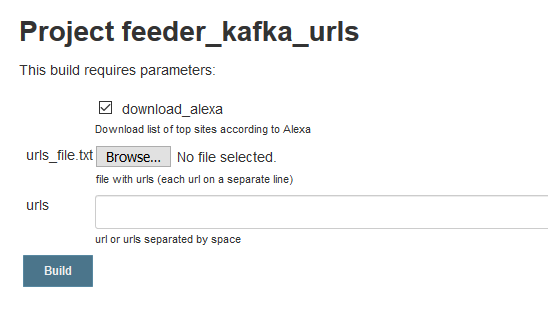
\includegraphics[width=8cm]{pictures/jenkins_kafka_feed.png}
	\caption{Parametry pro job \mintinline{Python}{feeder_kafka_urls}}
	\label{fig:kafka_feed}
\end{figure}

Prvním argumentem je parametr s názvem \mintinline{Python}{download_alexa}, který zajišťuje, že se před nahráním url do Kafky spustí kód pro stáhnutí top url stránek z listu na adrese \url{https://www.alexa.com/topsites}. Tato možnost je zaškrtnuta v základním nastavení (tzv. defaultně) a to z důvodu periodického spouštění tohoto jobu. Zbylé dva parametry jsou zde pro manuální spouštění. Prvním je možnost textového souboru \mintinline{Python}{urls_file.txt}, kdy uživatel může nahrát soubor s požadovaným listem webových adres, které chce stáhnout. Zbývá textový parametr \mintinline{Python}{urls}, kde se mohou adresy zadávat přímo do textového pole. Toho lze využít při potřebě stáhnout jen jednu požadovanou adresu. 

Skript využívá přístup do frontového systému Kafka. Bylo tedy zapotřebí v konfiguraci jobu nastavit požadované přístupové údaje. To je možné v konfigurační sekci Bindings, kde lze vytvořit tzv. environmentální proměnné (proměnná, která je přístupná odkudkoliv v celém prostředí) pro daný job. Takto byl nastavený SSL certifikát pro klienty Kafky a přístupové heslo pro autorizaci posílaných zpráv.

Konfigurace dále obsahuje sekci Build, v které je potřeba nastavit příkaz (tzv. command), který se má při spuštění provézt. Jedná se o command příkazové řádky operačního systému Windows, který spouští skript pro upload souborů do frontového systému Kafka v prostředí pythonu se zadanými parametry.



\subsubsection{Job pro stahování a filtraci dat} \label{sec:jenkinsvirt}
Druhým vytvořeným projektem v systému Jenkins je job pro spouštění zabezpečeného stahování a následné filtrování dat \mintinline{Python}{url_processing}. K tomu je zapotřebí virtuální stroj, který byl vytvořen v sekci \ref{sec:virtualka}. Tento job je spouštěn samostatně pro každou url, kterou dostává parametrem při spuštění. Tento parametr je předáván ze skriptu, který dostává zprávy z frontového systému Kafka. Ten je však spuštěn v systému Kubernetes. Proto byl v konfigurační sekci jobu vytvořen tzv. trigger token, tedy autorizační string. Pomocí tohoto stringu je možné tento job spouštět, a to pomocí dotazu na specifickou url adresu (viz \ref{trigger}).
\begin{equation} \label{trigger}
JENKINS\_URL/job/url\_processing/build?token=TOKEN
\end{equation}
$JENKINS\_URL$ značí webovou adresu serveru, na kterém běží firemní verze tohoto systému a $TOKEN$ je vygenerovaný autorizační řetězec znaků. Takto zadaný dotaz spustí job bez parametru. Pro předání parametru je nutné tento dotaz upravit,
\begin{equation}
.../url\_processing/BuildWithParameters?token=TOKEN\&url=URL
\end{equation}
kde $URL$ značí předávaný parametr url.

Je také nutné nastavit environmentální proměnné pro přihlašovací údaje do virtuálního systému. Toho je opět docíleno pomocí konfigurační sekce Bindings v nastavení jenkins projektu. 

Při startu jobu se spustí skript, který ovládá virtuální stroj. Toto je nastaveno v konfigurační sekci Build. Po úspěšném startu virtuálního stroje je ve virtuálním prostředí spuštěn klient pro stahování webového obsahu a následně jsou stažené soubory přeneseny zpět do prostředí jobu v Jenkinsu. Zde dochází k filtraci dat a soubory, které jsou vyhodnocené jako relevantní pro zadanou url adresu, jsou po doběhnutí jobu exportovány v podobě tzv. job artifactů (soubory, které jsou i po ukončení jobu dostupné). Tento export je proveden v konfigurační sekci Post-build Actions. Zde je také nastaveno, aby se po doběhnutí jobu spustil proces pro upload dat do databáze cleansetu (tzv. job trigger). Poněvadž jsou oba procesy v prostředí Jenkinsu, není potřeba generovat trigger token.






\subsubsection{Job pro upload dat do databáze cleansetu}
Třetím projektem vytvořeným v systému Jenkins je job pro upload do databáze cleansetu nazvaný \mintinline{Python}{scav_hcp_feeder}. Tento job nemá žádné vstupní parametry, využívá však exportované artifacty z jobu pro stahování a filtraci dat. Toto je nastaveno v konfigurační sekci Build (viz Obr.\ref{fig:jenkins_artifacts}). 

\begin{figure}[h]
	\centering
	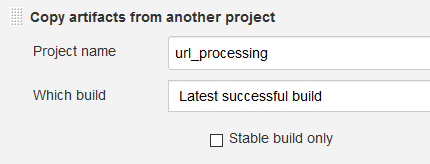
\includegraphics[width=8cm]{pictures/jenkins_artifacts.png}
	\caption{Přenos artifactů mezi joby}
	\label{fig:jenkins_artifacts}
\end{figure}

Parametr Project name určuje, z jakého projektu se mají exportované artifacty kopírovat, zde projekt \mintinline{Python}{url_processing}. Parametrem Which build lze přímo určit specifické číslo buildu projektu, z kterého se mají exportované artifacty získat. Lze také nastavit, aby se vždy braly z posledního úspěšného buildu, což je znázorněno na obrázku (viz Obr.\ref{fig:jenkins_artifacts}). Konfigurační sekce Build dále obsahuje příkaz pro spuštění samotného skriptu pro přenos těchto exportovaných souborů. 

Poněvadž se v jobu přistupuje do HCP úložiště, je potřeba v sekci Bindings nastavit environmentální proměnné obsahující přihlašovací údaje.



\subsection{Systém Kubernetes}\label{sec:luft}
V Kubernetes je spuštěn skript odebírající zprávy z frontového systému Kafka, který byl dockerizován. Dockerizace je proces vytvoření tzv. docker image (samostatně spustitelný balík v prostředí podporující funkcionalitu dockeru, např. Kubernetes). Tento balíček byl následně nahrán (tzv. deploy) do systému Kubernetes. Tím je docíleno neustálého běhu skriptu, což je pro tento typ programu praktické.



\subsubsection{Dockerizace skriptu Kafka consumer} 
Pro vytvoření docker image je nutné nejprve vytvořit tzv. Dockerfile (obdoba Makefile pro kompilaci jazyku C). Jedná se o soubor, který obsahuje sekvenci příkazů, které se mají při kompilaci docker balíčku provést. Dockerfile pro balíček obsahující skript Kafka consumer je znázorněn na snippetu \ref{snip:docker}.

\begin{figure}[h]               
	\begin{minted}{Docker}
FROM AVAST_DOCKER/python:3.7

COPY requirements.txt .

RUN pip install --no-cache-dir \
-r requirements.txt \
--index-url https://AVAST_ARTIFACTORY/pip/packages

ADD kafka_consumer_runner.py /
ADD lib/kafka_consumer.py /lib/
ADD config/config.py /config/

CMD ["python", "./kafka_consumer_runner.py"]
	\end{minted}      
	\caption{Dockerfile}
	\label{snip:docker}
\end{figure}

První řádek s příkazem \mintinline{Python}{FROM} určuje, odkud stáhnout tzv. image template (tj. docker balíček, který obsahuje prostředí, které se má při kompilaci docker kontejneru vytvořit). Protože je skript kafka consumer napsaný v Pythonu, je zapotřebí použít příslušný template. Kvůli bezpečnosti a pro zajištění integrity má firma vlastní úložiště s docker balíčky. Proto je balíček $python:3.7$ stažen z interního úložiště.

Dalším příkazem je překopírován soubor \mintinline{Python}{requirements.txt} do prostředí nově vzniklého kontejneru. Tento soubor obsahuje seznam nestandardních python knihoven, tedy knihoven, které je potřeba doinstalovat a nejsou obsaženy v instalaci pythonu.

Dále je spuštěn příkaz \mintinline{Python}{pip install}, který tyto nestandardní knihovny nainstaluje. K tomu je z bezpečnostních důvodů opět využito interní úložiště obsahující předschválené python knihovny.

Těmito příkazy je tedy připravené prostředí kontejneru. Zbývá přesunout zdrojové soubory skriptu, který zde poběží. Toho je docíleno příkazy \mintinline{Python}{ADD}. Posledním příkazem \mintinline{Python}{CMD} je spuštěn samotný skript.

Takto vytvořený Dockerfile je potřeba sestavit (tzv. build) a následně nasadit (tzv. deploy). K sestavení balíčku byl využit firemní server TeamCity (server pro kontinuální integraci a správu sestavování aplikací vyvíjený firmou JetBrains \cite{teamcity}). Zdejší firemní struktura obsahuje šablony pro build docker balíčků, které jsou následně nahrány do již zmíněného firemního úložiště.

Při nasazení aplikace do Kubernetes bylo opět využito firemní šablony. Při nasazování je potřeba vytvořit .yaml soubor, obsahující veškerou konfiguraci vznikající aplikace. Tento soubor byl převzat, bylo zde zapotřebí pouze nastavit environmentální proměnné, které skript využívá. Jednalo se o přihlašovací údaje a SSL certifikát k frontovému serveru Kafka a token, pomocí kterého skript spouští jenkins job pro stahování souborů (viz sekce \ref{sec:jenkinsvirt}).


\subsection{Schéma integrovaného systému}

Schéma \ref{fig:schema} znázorňuje celkové propojení systému Magpie. Skript Kafka Producer získává URL adresy a posílá je do frontového systému Kafka. Zde jsou adresy postupně odebírány skriptem Kafka Consumer, který pro každou adresu spouští job pro stahování souborů. Doběhnutím tohoto jobu je inicializován job pro HCP upload, kterému jsou stažené soubory (na diagramu znázorněny silnější šipkou) předány ve formě job artifactů. Soubory jsou nahrány do HCP úložiště a následně do Scavengeru.

\begin{figure}[h]
	\centering
	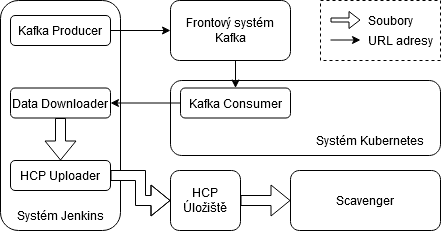
\includegraphics[width=11cm]{pictures/project_diagram.png}
	\caption{Diagram systému Magpie}
	\label{fig:schema}
\end{figure}








\chapter{Ověření funkčnosti}

\section{Testování}
Před nasazením aplikace do provozu bylo nutné zajistit důkladné otestování. Tento proces byl realizován formou end-to-end. Tato metoda kontroluje, zda je běh testované aplikace předpokládaný a zda aplikace vrací na zadaná vstupní data očekávané výstupy. Tento typ testování byl použit nejdříve pro jednotlivé komponenty, a následně pro celý běh aplikace. Komponenty, které byly při testování monitorovány, jsou následující:
\begin{itemize}
	\item Nahrávání adres do frontového systému Kafka
	\item Přijímání zpráv z Kafky a následná inicializace stahovacího procesu
	\item Zabezpečené stahování a filtrování dat
	\item Nahrávání validních dat do HCP úložistě 
\end{itemize}



\subsection{Komponenty využívající frontový systém Kafka}
Skripty pro komunikaci se systémem Kafka byly testovány již v průběhu vývoje, neočekávaly se zde tedy rozsáhlé komplikace. Při formě end-to-end byl zlomek testovacích adres v procesu Kafka Producer nahrán do Kafky a následně byly v procesu Kafka Consumer všechny adresy úspěšně přečteny. Následně byl proveden tzv. zatěžkávací test, tedy test, jehož snahou je určit, jak náročný provoz je daný systém schopný unést bez poruchy. Předpokládaná zátěž systému Magpie je v řádu tisíců až desetitisíců zpráv týdně. V zatěžkávacím testu byl tedy proveden přenos milionu zpráv. Tento přenos trval přibližně hodinu, což je v porovnání s předpokládanou zátěží více než dostačující propustnost. Následně byly všechny přijaté zprávy uloženy do souboru, jehož velikost byla porovnána se souborem obsahujícím vstupní data. Ze shody velikosti obou souborů bylo vyhodnoceno, že byl přenos úspěšný.


\subsection{Zabezpečené stahování a filtrování dat}
Testování této komponenty bylo nejobsáhlejší a probíhalo na vícero testovacích množinách. Prvotní testovací množina dat obsahovala 1000 vzorků a jednalo se o starší seznam nejnavštěvovaných url adres shromážděný službou Alexa top sites\cite{alexa}. Pro každou adresu byly staženy zdrojové soubory a následně byla provedena analýza výstupních dat. Při této analýze bylo zjištěno, že přes prvotní předpoklady není ošetření přesměrování se stavovými kódy 301 a 302 dostačující. Stavový kód 301 se používá pro trvalné přesměrování (tzv. Moved Permanently), kód 302 byl původně navržen pro dočasné přesměrování, nyní je nejčastěji používaným stavovým kódem pro obecná přesměrování. Z analýzy vyplynulo, že množství stránek používá i jiné stavové kódy pro přesměrování. Z ještě nezmíněných se nejčastěji objevoval kód 307, který od standardu HTTP/1.1 nahradil kód 302 pro dočasné redirecty (tzv. Temporary redirect). Proto bylo ošetření přesměrovávacích stavových kódů rozšířeno. Byl upraven inicializační skript(\ref{snip:fiddler}) pro program Fiddler, který obsahuje podmínku pro zachytávané stavové kódy (snippet \ref{snip:fiddler_new}). 

\begin{figure}[h]               
	\begin{minted}{Javascript}
if (code == 200 || code == 301 || code == 302)
	\end{minted}      
	\caption{Původní podmínka selekce stavových kódů}
	\label{snip:fiddler_new}
\end{figure}

Zmiňovaná podmínka byla rozšířena na zachytávání všech stavových kódů z intervalu $(300,308)$ včetně (znázorněno na snippetu \ref{snip:fiddler_new_new}).
\begin{figure}[h]               
	\begin{minted}{Javascript}
if (oSession.responseCode == 200 || 
    (300 <= oSession.responseCode <= 308))
	\end{minted}      
	\caption{Upravená podmínka selekce stavových kódů}
	\label{snip:fiddler_new_new}
\end{figure}

Z analýzy následně vyplynula důležitost uchovávání logu (výpis informačních zpráv) prohlížeče. Tento výpis je důležitý v situacích, kdy zadaná stránka již neexistuje, nebo se v průběhu připojení naskytly jiné komplikace a obsah stránky není dostupný. V takovém případě není nutné pokračovat třídícím algoritmem, poněvadž všechny zachycené soubory obsahují pouze režijní komunikaci prohlížeče a Fiddleru. Geckodriver (webdriver používaný nástrojem Selenium k ovládání internetového prohlížeče Mozilla Firefox) ovšem tuto funkcionalitu nepodporuje. Z toho důvodu bylo od těchto nástrojů odstoupeno a byl použit Chromedriver v souvislosti s internetovým prohlížečem Google Chrome. K tomu bylo zapotřebí na virtuální stroj nainstalovat zmíněný webdriver ve verzi shodné s nainstalovaným prohlížečem Google Chrome (pro oba programy byla nainstalována nejnovější verze 80). Základní ovládání prohlížeče se liší pouze v importování a následné inicializaci rozdílné třídy reprezentující prohlížeč z knihovny nástroje Selenium. Kód pro ovládání prohlížeče nástrojem Selenium \ref{snip:selenium} byl tedy přepsán. Základní ovládání prohlížeče Google Chrome s využitím logování je znázorněno na snippetu \ref{snip:selenium_new}.

\begin{figure}[h]               
	\begin{minted}{Python}
import time 

from selenium.webdriver import Chrome
import selenium.webdriver.common.desired_capabilities
import selenium.webdriver

chrome_options = selenium.webdriver.ChromeOptions()

d = desired_capabilities.DesiredCapabilities.CHROME
d['goog:loggingPrefs'] = {'browser': 'ALL'}

browser = Chrome(
    options=chrome_options, 
    desired_capabilities=d
)

browser.get("https://www.seznam.cz")
log = browser.get_log('browser')
	\end{minted}      
	\caption{Ovládání prohlížeče Google Chrome pomocí nástroje Selenium}
	\label{snip:selenium_new}
\end{figure}

Obdobně jako u prohlížeče Firefox lze měnit nastavení prohlížeče skrze instanci dedikované třídy, zde \mintinline{Python}{ChromeOptions}. Dále je potřeba vytvořit instanci třídy \mintinline{Python}{DesiredCapabilities}, v které je možné nastavit logovací preference(\ref{snip:log_pref}).
\begin{figure}[h]               
	\begin{minted}{Python}
d['goog:loggingPrefs'] = {'browser': 'ALL'}
	\end{minted}      
	\caption{Logovací preference prohlížeče}
	\label{snip:log_pref}
\end{figure}
Parametr \mintinline{Python}{'ALL'} určuje úroveň logování, tedy zda se mají ukládat všechny informační zprávy (ALL), nebo jen zprávy typu ERROR či WARNING.
Tato instance je předána spolu s třídou pro nastavení prohlížeče jako parametry při inicializaci prohlížeče. Po načtění stránky lze přistoupit k logu pomocí metody \mintinline{Python}{get_log()}, která vrací strukturu obsahující informace v závislosti na nastavených logovacích preferencích. Při iteraci nad touto strukturou lze přistoupit k jednotlivým záznamům (snippet \ref{snip:selenium_logger}). 
\begin{figure}[h]               
	\begin{minted}{Python}
for entry in log:
    print(f"{entry['message']}")
    if 'Fiddler - DNS Lookup Failed' in entry['message']:
        raise DNSLookUpFailException(entry['message'])
    if 'Fiddler - Connection Failed' in entry['message']:
        raise ConnectionFailException(entry['message'])
    if 'Fiddler - Receive Failure' in entry['message']:
        raise ReceiveFailureException(entry['message'])
	\end{minted}      
	\caption{Iterace nad strukturou obsahující logování prohlížeče}
	\label{snip:selenium_logger}
\end{figure}

Tento výpis byl následně použit k vytvoření podmínek kontrolujících, zda byla stránka skutečně načtena. Chybové hlášky prohlížeče nejsou nijak exaktní, bylo tedy nutné podmínky vytvořit na základě porovnávání stringů. Z analýzy vyplynulo, že se při neexistující stránce nebo při přerušeném připojení objevují tři rozdílné výpisy. Byly tedy vytvořeny podmínky, které tyto výpisy odchytávají a vytvářejí výjimky, které se na začátku procesu filtrování dat vyhodnocují.


\subsection{Přenos souborů do HCP úložiště}
Posledním krokem testování byl klient pro HCP úložiště. Samotná komunikace s úložištěm je zajištěna pomocí knihovny vytvořené týmem spravujícím systém Scavenger, tuto funkcionalitu tedy testovat nutné nebylo. V testovacím procesu bylo převážně kontrolováno správné přikládání metadat k nahrávaným souborům. K testování byl opět využit starší seznam nejnavštěvovaných url adres shromážděný službou Alexa top sites\cite{alexa} o velikosti 1000 vzorků. Jelikož je přenos závislý na stažených datech, byly tyto vzorky nejdříve zpracovány komponentou pro stahování a filtraci dat. Soubory, které byly v tomto kroku vyhodnocené jako validní, byly spolu s jejich metadaty nahrány do HCP úložiště a následně byla provedena kontrola nahraných dat. Metadata nahraných souborů byla porovnána se staženými metadaty a ve všech případech byla shledána shoda. Z toho bylo vyvozeno, že přikládání metadat k nahrávaným souborům funguje v pořádku. 

Při této analýze bylo avšak zjištěno, že přejmenovávání nahraných souborů podle klíče
\begin{center}\label{prej}
\{původní\_adresa\}\{pořadí\_zpracovaného\_souboru\}
\end{center}
 není optimální. V HCP úložišti mohou být pouze soubory s unikátním názvem. K přenosu souborů z HCP úložiště do systému Scavenger nedochází hned, avšak periodicky s časovým odstupem. V situaci, kdy by v tomto čase byla zpracována stejná url adresa vícekrát, by došlo k pokusu o nahrání souboru, který by měl stejné jméno jako soubor již přítomný v HCP úložišti, a přenos by neproběhl. Bylo tedy nutné klíč přetvořit, aby byla zachována unikátnost. K tomuto účelu je k názvu souboru přidáván i současný čas. Nový klíč pro přejmenovávání nahrávaných souborů tedy vypadá následovně: 
\begin{center}\label{prejm}
\{původní\_adresa\}\{pořadí\_zpracovaného\_souboru\}\{aktuální\_čas\}
\end{center}

Dále byla na začátek přenosu přidána kontrola, zda při filtraci dat byly vůbec některé soubory označeny jako validní. Pokud tomu tak není, proces se automaticky ukončí.


\section{Monitorování}\label{monitoring}
K monitorování funkčnosti aplikace byl využit analytický nástroj Grafana\cite{grafana} v kombinaci s databázovým systémem Graphite\cite{graphite}, který uchovává data s časovou známkou. Tato data je následně možné znázorňovat ve formě grafů pomocí nástroje Grafana. K posílání dat do systému Graphite byla využita python knihovna \textit{Statsd}\cite{statistika}.

Při chodu aplikace jsou monitorovány údaje o stažených souborech (počet souborů a jejich velikost) spolu s úspěšností zpracování zadaných adres. 

\begin{figure}[h]
	\centering
	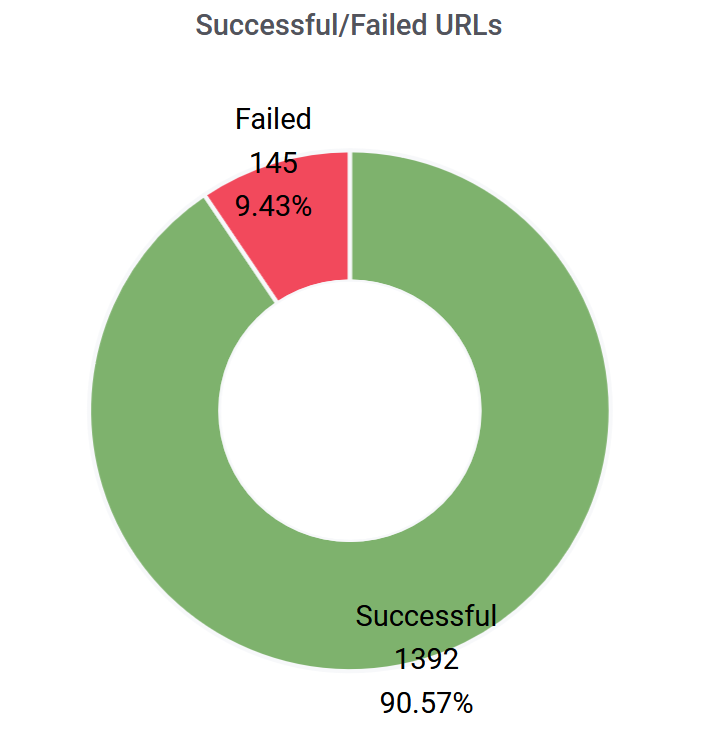
\includegraphics[width=5cm]{pictures/URLgraph.png}
	\caption{Zpracované adresy v rámci jednoho dne}
	\label{fig:urls}
\end{figure}

Na grafu \ref{fig:urls} je zachycen podíl úspěšně zpracovaných adres v rámci jednoho dne. Z grafu je patrné, že systém Magpie je schopný za jeden den zpracovat přibližně 1500 zadaných adres, z čehož je přibližně 90\% úspěšně. Ve zbylých případech nebylo možné navázat spojení z požadovanou adresou. Tato  desetiprocentní neúspěšnost systému je dána vstupními daty. Jelikož se zpracovávají globálně nejnavštěvovanější adresy podle serveru Majestic Milion, je velice pravděpodobné, že se v těchto seznamech objeví adresy, které jsou již nefunkční, zablokované či jinak nedostupné. I přesto je systém Magpie schopný úspěšně zpracovávat až 1400 adres denně.

Graf \ref{fig:files2} znázornuje počet stažených souborů za minutu v rámci jednoho dne. Interval minuty je daný nástrojem Graphite, který data takto automaticky agreguje. Z grafu je patrná funčnost systému s průměrem přibližně čtyřiceti stažených souborů za minutu. V rámci jednoho dne je tedy možné získat až 50 tisíc souborů, z čehož je přibližně 15 tisíc unikátních.


\begin{figure}[h]
	\centering
	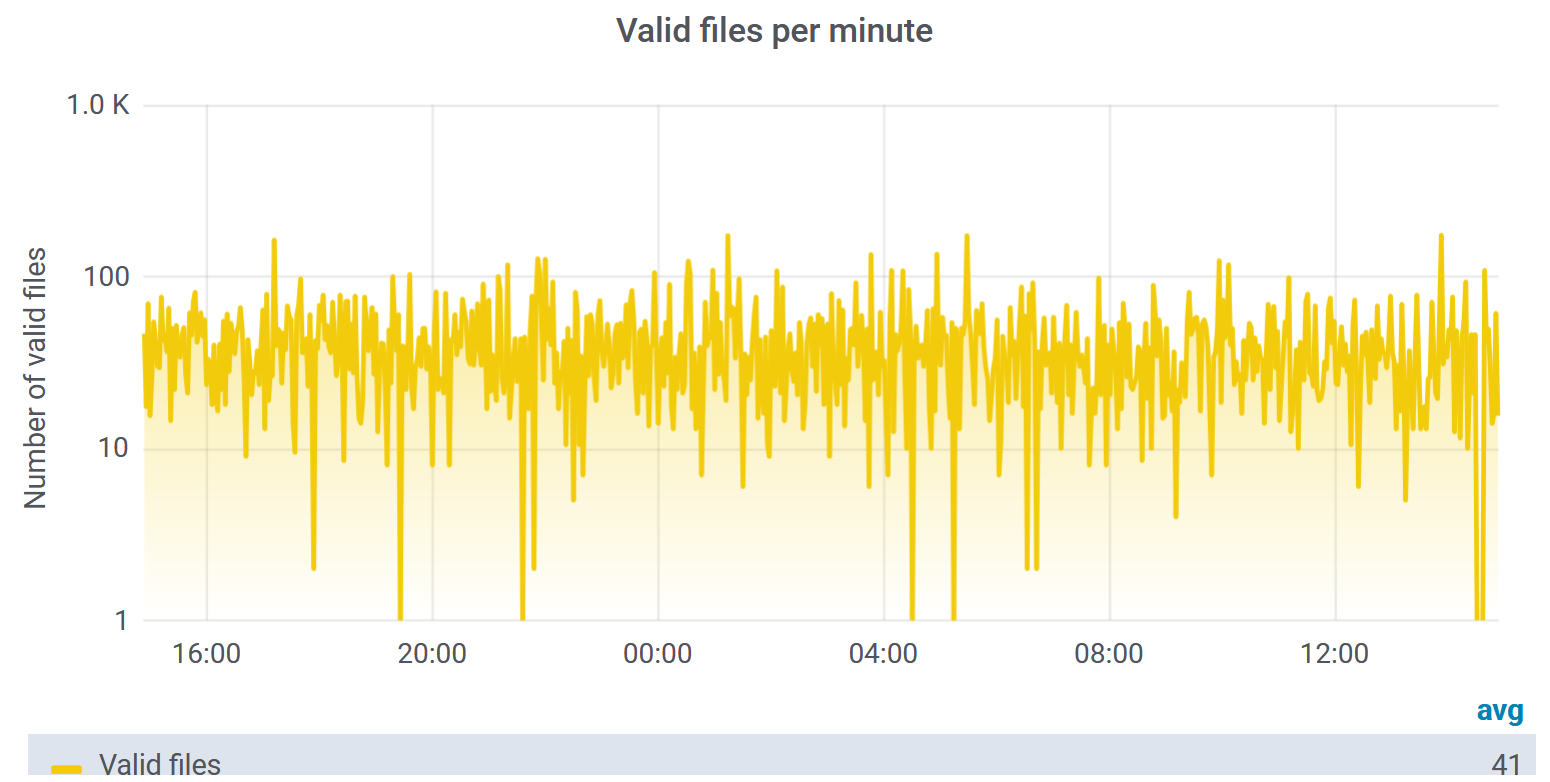
\includegraphics[width=12cm]{pictures/files3.png}
	\caption{Počet stažených souborů v rámci jednoho dne}
	\label{fig:files2}
\end{figure}


\chapter{Přínos a budoucí využití}
\section{Zobecnění projektu a budoucí využití}
V současné době je projekt Magpie využíván k doplňování cleansetu stahováním zdrojových souborů webových stránek s vysokou prevalencí. Při vývoji se ale již počítalo s jeho širším využitím v jiných aplikacích potřebujících zabezpečený zisk zdrojových souborů. Jedním z takových případů může být analýza phishingových stránek. Jedná se o stránky, které využívají nepozornosti uživatele k zisku citlivých informací. Při analýze těchto stránek, tedy při rozhodování, zda je stránka phishingového charakteru, je často potřeba podívat se do zdrojových souborů stránky. K zisku těchto dat by bylo možné využívat systém Magpie. 

Jiným využitím Magpie při analýze malwaru může být zisk infikovaných souborů s následným nahráním do systému Scavenger. Systém Scavenger obsahuje kromě databáze cleansetu mimojiné i databázi škodlivých souborů. Rozhodovací logika vložení nahrávaného souboru do příslušné databáze je lehce implementovatelná v systému Scavenger pomocí filterů založených na metadatech nahrávaných souborů. Pokud by byla tedy metadata obohacena o tuto informaci, je Magpie schopný zpracovávat i infikovaná data. Této funkcionalitě značně přispívá fakt, že je jádro projektu realizováno ve virtuálním prostředí, což umožňuje zabezpečené stahování nejen čistých souborů.



\section{Zhodnocení přínosu}
Hlavní přínos systému Magpie je v automatizaci doplňování cleansetu. Dříve bylo doplňování čistých či infikovaných html a js souborů do databáze Scavengeru prací analytiků, kteří museli pro každý nahraný soubor manuálně zvolit, zda se jedná o soubor infikovaný či nikoliv. Tímto způsobem není možné zpracovávat obsáhlý počet čistých souborů, které je třeba nahrávat na cleanset, aby byla zajištěna jeho funkčnost. Díky systému Magpie je možné cleanset obohacovat o desetitisíce nových souborů týdně, čímž je mnohonásobně navýšena stávající frekvence přidávání dat. Toto je zobrazeno na grafu \ref{fig:scav}, který zachycuje frontu v systému Scavenger s nově přidanými soubory na cleanset v rámci jednoho dne. Zde je vidět, že systém Magpie obohacuje cleanset o řádově stovky unikátních souborů každou hodinu jeho provozu. 

\begin{figure}[h]
	\centering
	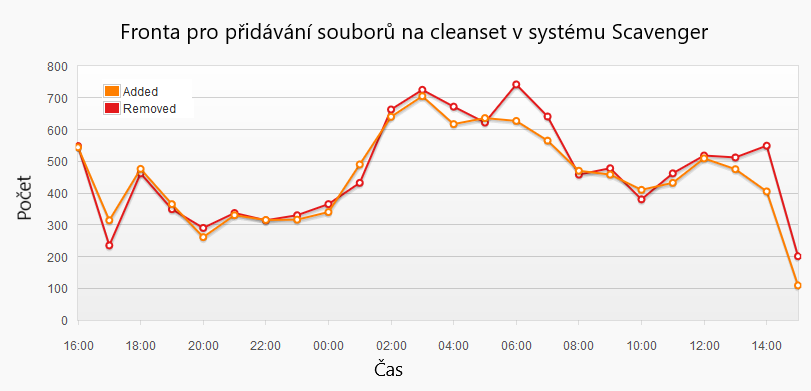
\includegraphics[width=12cm]{pictures/scav.png}
	\caption{Unikátní soubory přidané do systému Scavenger}
	\label{fig:scav}
\end{figure}

V důsledku toho je cleanset obsáhlejší, což přispívá k lépe fungující automatizaci při vydávání nových detekcí. Virové detekce vytvářejí analytici, kteří musí kontrolovat, zda detekce neblokuje čisté soubory na cleansetu. Virové detekce zároveň vznikají i díky automatickým nástrojům, u kterých je silný cleanset neméně důležitý. Díky silnému cleansetu klesá množství špatných detekcí vytvořených automatickými nástroji a Magpie takovýto cleanset vytváří.







 \setlength{\parskip}{10pt}





\begin{conclusion}

Diplomová práce spočívala ve vytvoření automatizovaného systému pro obohacování cleansetu o čisté html a js soubory stahováním těchto souborů ze zadaných url adres. Prvním bodem zadání byla analýza možných způsobů realizace tohoto systému. Během této analýzy bylo zjištěno, jaké jsou nejlepší postupy při realizaci projektu. 

Na základě toho byl vytvořen projekt Magpie. Projekt byl navržen v programovacím jazyku Python a je rozdělen do několika komponent. Pro předzpracování vstupních dat byl vytvořen skript využívající frontový systém Apache Kafka. Pomocí skriptu je možné zpracovávat seznamy url adres služby Alexa Top Sites, či ručně zadané adresy. Tento skript je nasazen v systému Jenkins. Dále byl vytvořen skript pro čtení zpráv z frontového systému Kafka. Tento skript byl dockerizován a nasazen v systému Kubernetes. Jádro projektu spočívá ve stahování dat pomocí MitM klientu Fiddler v kombinaci s internetovým prohlížečem Google Chrome ovládaným pomocí nástroje Selenium. Tento proces je spouštěn na virtuálním stroji s využitím programu Oracle Virtualbox a nasazen v systému Jenkins. Stažená data jsou odesílána do HCP úložiště a následně nahrána do databáze cleansetu v systému Scavenger, k čemuž slouží poslední komponenta také nasazená v systému Jenkins.

Dalším bodem zadání bylo zobecnění vzniklého systému pro budoucí využití v jiných projektech. Se zobecněním bylo počítáno již při samotném návrhu hlavní aplikace. Systém Magpie je schopný zpracovávat nejen adresy pro stahování dat k doplňování cleansetu. Toho bude v budoucnu využito při analýze phishingových i jinak potenciálně nebezpečných url adres.

Posledním bodem zadání bylo důsledné otestování navrženého systému. Testování proběhlo na vícero testovacích množinách s využitím seznamu adres služby Alexa Top Sites. Každá komponenta byla otestována zvlášt a nakonec bylo využito i end-to-end testování celé aplikace.

Díky systému Magpie je nyní možné rozšiřovat cleanset o desetitísice nových souborů týdně, což je oproti dosavadnímu ručnímu rozšiřování výrazné zlepšení. 







\end{conclusion}


\bibliographystyle{csn690}
\bibliography{mybibliographyfile}
\begin{thebibliography}{9}

    \bibitem{avast_flier}
    Avast corporate factsheet. \textit{Avast Software} [online]. Copyright ©2019, Avast Software [cit. 14.04.2020]. Dostupné z: \\       \url{https://cdn2.hubspot.net/hubfs/2706737/media-materials/corporate-factsheet/Avast_corporate_factsheet_A4_en.pdf}
       	
    
    \bibitem{python}
    
    Welcome to Python.org. \textit{Welcome to Python.org} [online]. Copyright ©2001 [cit. 14.04.2020]. Dostupné z: \\ 
     \url{https://www.python.org/}
    
    \bibitem{fiddler}   
    
    Fiddler - Free Web Debugging Proxy - Telerik. \textit{Telerik UI for ASP.NET AJAX, MVC, Core, Xamarin, Angular, HTML5 and jQuery} [online]. Copyright © 2020, Progress Software Corporation and [cit. 14.04.2020]. Dostupné z:  \\ 
    \url{https://www.telerik.com/fiddler}
    
    \bibitem{beautifulsoup}
    Beautiful Soup: We called him Tortoise because he taught us.. \textit{Swear not by the wiki, the fickle wiki, the inconstant wiki} [online]. Copyright © 1996 [cit. 14.04.2020]. Dostupné z:     \\  \url{https://www.crummy.com/software/BeautifulSoup/} 	

    
    \bibitem{mitm}
    What is MITM (Man in the Middle) Attack | Imperva. \textit{Cyber Security Leader | Imperva, Inc.} [online]. Copyright © 2020 Imperva. All rights reserved [cit. 14.04.2020]. Dostupné z:  \\ 
    \url{https://www.imperva.com/learn/application-security/man-in-the-middle-attack-mitm/}


	\bibitem{kafka}
	Overview of Kafka. In: \textit{Wikipedia: the free encyclopedia} [online]. San Francisco (CA): Wikimedia Foundation, 2001- [cit. 2020-04-14]. Dostupné z: \\ 
	\url{https://en.wikipedia.org/wiki/Apache_Kafka#/media/File:Overview_of_Apache_Kafka.svg}
	
	\bibitem{virutalbox}
	Oracle VM VirtualBox. User Manual v6.1.4. \textit{Oracle Corporation} [online]. Copyright © 2020 Oracle Corporation [cit. 14.04.2020]. Dostupné z: \\ 
	\url{http://download.virtualbox.org/virtualbox/UserManual.pdf}
	
	\bibitem{docker}	
	What is a Container? | App Containerization | Docker. \textit{Empowering App Development for Developers | Docker} [online]. Copyright © 2020 Docker Inc. All rights reserved [cit. 14.04.2020]. Dostupné z: \\ 
	\url{https://www.docker.com/resources/what-container}
	
	\bibitem{vbox_pic}
	Virtualizace na desktopu. \textit{Michal Zobec: Virtuální PC Blog} [online]. Dostupné z: \\  
	\url{https://www.virtualnipc.cz/wp-content/gallery/140701-1-uvod-do-virtualizace-na-desktopu/cache/140701-uvod-do-virtualizace-na-desktopu-img-1.png-nggid013-ngg0dyn-640x480x100-00f0w010c010r110f110r010t010.png}
	
	\bibitem{vmware}
	vSphere Automation SDK for Python. \textit{VMware Inc.} [online]. Copyright ©2020 VMware, Inc. [cit. 14.04.2020]. Dostupné z:  \\ 
	\url{https://code.vmware.com/web/sdk/6.7/vsphere-automation-python}
	
	\bibitem{pyvbox}
	pyvbox Documentation. \textit{Dorman Michael} [online]. Copyright \textcopyright2017 Dostupné z: \\ 
	\url{https://buildmedia.readthedocs.org/media/pdf/pyvbox/latest/pyvbox.pdf}
	
	\bibitem{gecko}
	Releases · mozilla/geckodriver · GitHub. \textit{The world’s leading software development platform · GitHub} [online]. Copyright © 2020 GitHub, Inc. [cit. 14.04.2020]. Dostupné z:  \\ 
	\url{https://github.com/mozilla/geckodriver/releases}
	
	\bibitem{firefox}
	Firefox Browser. \textit{Mozilla} [online]. Copyright ©1998-2020 [cit. 14.04.2020]. Dostupné z:  \\ 
	\url{https://www.mozilla.org/cs/firefox/new/}
	
	\bibitem{chrome}
	Webový prohlížeč Google Chrome. \textit{Google} [online]. [cit. 14.04.2020]. Dostupné z:  \\ 
	\url{https://www.google.com/intl/cs_CZ/chrome/}
	
	\bibitem{chromedriver}
	ChromeDriver - WebDriver for Chrome. \textit{ChromeDriver - WebDriver for Chrome} [online]. [cit. 14.04.2020]. Dostupné z: \\ 
	\url{https://chromedriver.chromium.org/}
	
	\bibitem{hcp}	
	Hitachi Content Platform (HCP) - Harness Data Growth. \textit{Hitachi Vantara.} [online]. [cit. 14.04.2020]. Dostupné z: \\ https://www.hitachivantara.com/en-us/products/storage/object-storage/content-platform.html
	
	\bibitem{response_codes}
	HTTP/1.1: Status Code Definitions. \textit{World Wide Web Consortium (W3C)} [online]. [cit. 14.04.2020]. Dostupné z: \\ 
	\url{https://www.w3.org/Protocols/rfc2616/rfc2616-sec10.html}
	
	\bibitem{confluent-kafka}
	Kafka Python Client — Confluent Platform. \textit{Confluent} [online]. Copyright ©2020 [cit. 14.04.2020]. Dostupné z:  \\ 
	\url{https://docs.confluent.io/current/clients/python.html}
	
	\bibitem{teamcity}
	TeamCity: the Hassle-Free CI and CD Server by JetBrains. \textit{JetBrains: Developer Tools for Professionals and Teams} [online]. [cit. 14.04.2020]. Dostupné z: \\ 
	\url{https://www.jetbrains.com/teamcity/}
	
	\bibitem{alexa}
	Alexa - Top sites. \textit{Alexa - Keyword Research, Competitive Analysis and Website Ranking} [online]. Copyright © Alexa Internet, Inc. 1996 [cit. 14.04.2020]. Dostupné z:  \\ 
	\url{https://www.alexa.com/topsites}
	
	\bibitem{majestic}
	The Majestic Million. \textit{SEO Backlink Checker and Link Building Toolset | Majestic.com} [online]. [cit. 14.04.2020]. Dostupné z:  \\ 
	\url{https://majestic.com/reports/majestic-million}
	
	\bibitem{grafana}
	Grafana. \textit{Grafana Labs} [online]. Copyright 2020 © Grafana Labs [cit. 14.04.2020]. Dostupné z: \\
	\url{https://grafana.com/}
	
	\bibitem{graphite}	
	Graphite. Graphite [online]. [cit. 14.04.2020]. Dostupné z: \\
	\url{https://graphiteapp.org/}
	
	
	\bibitem{statistika}	
	statsd · PyPI. \textit{PyPI · The Python Package Index} [online]. Copyright © 2020 [cit. 14.04.2020]. Dostupné z: \\
	\url{https://pypi.org/project/statsd/}
	
	\bibitem{book1}
	Eric Lawrence, CreateSpace Independent Publishing Platform (2015).\textit{ Debugging with
	Fiddler: The complete reference from the creator of the Fiddler Web Debugger, 2nd
	Edition.} ISBN: 9781511572903.
	
	\bibitem{book2}
	Ryan Mitchell, O'Reilly Media, Inc. (2018). \textit{Web Scraping with Python, 2nd Edition.}
	ISBN: 9781491985564.
	
	\bibitem{book3}
	Harry Colvin, CreateSpace Independent Publishing Platform (2015). \textit{VirtualBox: An
	Ultimate Guide Book on Virtualization with VirtualBox.} ISBN: 1522769889.
		
\end{thebibliography}

\appendix

%\begin{figure}[h]               
%	\begin{minted}{c}
%	code
%	\end{minted}      
%	\caption{Implementace bloku PI regulátor v jazyce C}
%	\label{fig:ctrl.c}
%\end{figure}

%\begin{figure}[h]               
%	\begin{minted}{Java}
%	code
%	\end{minted}      
%	\caption{Deklarace nativní metody a načtení sdílené knihovny}
%	\label{fig:SISO.java}
%\end{figure}

% \begin{figure}[h]
%         \centering
%         \begin{minipage}[b]{0.49\textwidth}
%                 \includegraphics[width=6cm]{pictures/car2.JPG}
%                 \caption*{(a) Pohled po odmontování kapoty}
%                 \label{fig:car2}
% 		\end{minipage}
%         \begin{minipage}[b]{0.49\textwidth}
%                 \includegraphics[width=6cm]{pictures/car3.JPG}
%                 \caption*{(b) Spodní STM modul a DC motor}
%                 \label{fig:car1}
%         \end{minipage}
% 	\caption{Vnitřek vozidel}
% 	\label{fig:cars}
% \end{figure}

\chapter{Seznam použitých zkratek}
 \printglossaries
\begin{description}
	\item[AJAX] Asynchronous JavaScript and XML
	\item[API] Application programming interface
	\item[CI/CD] Continuous integration/continuous delivery
	\item[CSS] Cascading style sheet
	\item[GUI] Graphical user interface
	\item[HCP] Hitachi content platform
	\item[HTML] Hypertext markup language
	\item[HTTP] Hypertext transfer protocol
	\item[JS] JavaScript
	\item[MitM] Man in the middle
	\item[OS] Operating system
	\item[PaaS] Platform as a service
	\item[SDK] Software development kit
	\item[SHA] Secure hash algorithm
	\item[SMB] Server message block
	\item[SSL] Secure sockets layer
	\item[URL] Uniform resource locator
	\item[VBOX] VirtualBox
	\item[VM] Virtual machine
	\item[XML] Extensible markup language
\end{description}


% % % % % % % % % % % % % % % % % % % % % % % % % % % % 
% % Tuto kapitolu z výsledné práce ODSTRAŇTE.
% % % % % % % % % % % % % % % % % % % % % % % % % % % % 
% 
% \chapter{Návod k~použití této šablony}
% 
% Tento dokument slouží jako základ pro napsání závěrečné práce na Fakultě informačních technologií ČVUT v~Praze.
% 
% \section{Výběr základu}
% 
% Vyberte si šablonu podle druhu práce (bakalářská, diplomová), jazyka (čeština, angličtina) a kódování (ASCII, \mbox{UTF-8}, \mbox{ISO-8859-2} neboli latin2 a nebo \mbox{Windows-1250}). 
% 
% V~české variantě naleznete šablony v~souborech pojmenovaných ve formátu práce\_kódování.tex. Typ může být:
% \begin{description}
% 	\item[BP] bakalářská práce,
% 	\item[DP] diplomová (magisterská) práce.
% \end{description}
% Kódování, ve kterém chcete psát, může být:
% \begin{description}
% 	\item[UTF-8] kódování Unicode,
% 	\item[ISO-8859-2] latin2,
% 	\item[Windows-1250] znaková sada 1250 Windows.
% \end{description}
% V~případě nejistoty ohledně kódování doporučujeme následující postup:
% \begin{enumerate}
% 	\item Otevřete šablony pro kódování UTF-8 v~editoru prostého textu, který chcete pro psaní práce použít -- pokud můžete texty s~diakritikou normálně přečíst, použijte tuto šablonu.
% 	\item V~opačném případě postupujte dále podle toho, jaký operační systém používáte:
% 	\begin{itemize}
% 		\item v~případě Windows použijte šablonu pro kódování \mbox{Windows-1250},
% 		\item jinak zkuste použít šablonu pro kódování \mbox{ISO-8859-2}.
% 	\end{itemize}
% \end{enumerate}
% 
% 
% V~anglické variantě jsou šablony pojmenované podle typu práce, možnosti jsou:
% \begin{description}
% 	\item[bachelors] bakalářská práce,
% 	\item[masters] diplomová (magisterská) práce.
% \end{description}
% 
% \section{Použití šablony}
% 
% Šablona je určena pro zpracování systémem \LaTeXe{}. Text je možné psát v~textovém editoru jako prostý text, lze však také využít specializovaný editor pro \LaTeX{}, např. Kile.
% 
% Pro získání tisknutelného výstupu z~takto vytvořeného souboru použijte příkaz \verb|pdflatex|, kterému předáte cestu k~souboru jako parametr. Vhodný editor pro \LaTeX{} toto udělá za Vás. \verb|pdfcslatex| ani \verb|cslatex| \emph{nebudou} s~těmito šablonami fungovat.
% 
% Více informací o~použití systému \LaTeX{} najdete např. v~\cite{wikilatex}.
% 
% \subsection{Typografie}
% 
% Při psaní dodržujte typografické konvence zvoleného jazyka. České \uv{uvozovky} zapisujte použitím příkazu \verb|\uv|, kterému v~parametru předáte text, jenž má být v~uvozovkách. Anglické otevírací uvozovky se v~\LaTeX{}u zadávají jako dva zpětné apostrofy, uzavírací uvozovky jako dva apostrofy. Často chybně uváděný symbol "{} (palce) nemá s~uvozovkami nic společného.
% 
% Dále je třeba zabránit zalomení řádky mezi některými slovy, v~češtině např. za jednopísmennými předložkami a spojkami (vyjma \uv{a}). To docílíte vložením pružné nezalomitelné mezery -- znakem \texttt{\textasciitilde}. V~tomto případě to není třeba dělat ručně, lze použít program \verb|vlna|.
% 
% Více o~typografii viz \cite{kobltypo}.
% 
% \subsection{Obrázky}
% 
% Pro umožnění vkládání obrázků je vhodné použít balíček \verb|graphicx|, samotné vložení se provede příkazem \verb|\includegraphics|. Takto je možné vkládat obrázky ve formátu PDF, PNG a JPEG jestliže používáte pdf\LaTeX{} nebo ve formátu EPS jestliže používáte \LaTeX{}. Doporučujeme preferovat vektorové obrázky před rastrovými (vyjma fotografií).
% 
% \subsubsection{Získání vhodného formátu}
% 
% Pro získání vektorových formátů PDF nebo EPS z~jiných lze použít některý z~vektorových grafických editorů. Pro převod rastrového obrázku na vektorový lze použít rasterizaci, kterou mnohé editory zvládají (např. Inkscape). Pro konverze lze použít též nástroje pro dávkové zpracování běžně dodávané s~\LaTeX{}em, např. \verb|epstopdf|.
% 
% \subsubsection{Plovoucí prostředí}
% 
% Příkazem \verb|\includegraphics| lze obrázky vkládat přímo, doporučujeme však použít plovoucí prostředí, konkrétně \verb|figure|. Například obrázek \ref{fig:float} byl vložen tímto způsobem. Vůbec přitom nevadí, když je obrázek umístěn jinde, než bylo původně zamýšleno -- je tomu tak hlavně kvůli dodržení typografických konvencí. Namísto vynucování konkrétní pozice obrázku doporučujeme používat odkazování z~textu (dvojice příkazů \verb|\label| a \verb|\ref|).
% 
% \begin{figure}\centering
% 	
\includegraphics[width=0.5\textwidth, angle=30]{cvut-logo-bw}
% 	\caption[Příklad obrázku]{Ukázkový obrázek v~plovoucím prostředí}\label{fig:float}
% \end{figure}
% 
% \subsubsection{Verze obrázků}
% 
% % Gnuplot BW i barevně
% Může se hodit mít více verzí stejného obrázku, např. pro barevný či černobílý tisk a nebo pro prezentaci. S~pomocí některých nástrojů na generování grafiky je to snadné.
% 
% Máte-li například graf vytvořený v programu Gnuplot, můžete jeho černobílou variantu (viz obr. \ref{fig:gnuplot-bw}) vytvořit parametrem \verb|monochrome dashed| příkazu \verb|set term|. Barevnou variantu (viz obr. \ref{fig:gnuplot-col}) vhodnou na prezentace lze vytvořit parametrem \verb|colour solid|.
% 
% \begin{figure}\centering
% 	\includegraphics{gnuplot-bw}
% 	\caption{Černobílá varianta obrázku generovaného programem Gnuplot}\label{fig:gnuplot-bw}
% \end{figure}
% 
% \begin{figure}\centering
% 	\includegraphics{gnuplot-col}
% 	\caption{Barevná varianta obrázku generovaného programem Gnuplot}\label{fig:gnuplot-col}
% \end{figure}
% 
% 
% \subsection{Tabulky}
% 
% Tabulky lze zadávat různě, např. v~prostředí \verb|tabular|, avšak pro jejich vkládání platí to samé, co pro obrázky -- použijte plovoucí prostředí, v~tomto případě \verb|table|. Například tabulka \ref{tab:matematika} byla vložena tímto způsobem.
% 
% \begin{table}\centering
% 	\caption[Příklad tabulky]{Zadávání matematiky}\label{tab:matematika}
% 	\begin{tabular}{|l|l|c|c|}\hline
% 		Typ		& Prostředí		& \LaTeX{}ovská zkratka	& \TeX{}ovská zkratka	\tabularnewline \hline \hline
% 		Text		& \verb|math|		& \verb|\(...\)|	& \verb|$...$|		\tabularnewline \hline
% 		Displayed	& \verb|displaymath|	& \verb|\[...\]|	& \verb|$$...$$|	\tabularnewline \hline
% 	\end{tabular}
% \end{table}
% 
% % % % % % % % % % % % % % % % % % % % % % % % % % % % 

\chapter{Obsah přiloženého CD}

%upravte podle skutecnosti

\begin{figure}
	\dirtree{%
		.1 Magpie\DTcomment{adresář s Python projektem}.
		.2 config.
		.3 config.py\DTcomment{configurační soubor}.
		.2 lib.
		.3 files\_filter.py\DTcomment{metody pro filtrování dat}.
		.3 hcp\_feeder.py\DTcomment{metody pro HCP komunikaci}.
		.3 kafka\_consumer.py\DTcomment{implementace klientu Kafka consumer}.
		.3 kafka\_producer.py\DTcomment{implementace klientu Kafka producer}.
		.3 logger.py\DTcomment{implementace logování}.
		.3 tools.py\DTcomment{metody pro obecné nástroje}.
		.3 virtualbox\_handler.py\DTcomment{metody pro program VirtualBox}.
		.2 vbox\_scripts.
		.3 browser\_controller.py\DTcomment{skript spouštěný ve virtuálním prostředí}.
		.3 CustomRules.js\DTcomment{inicializační skript prograu Fiddler}.
		.2 Dockerfile\DTcomment{dockerizační skript}.
		.2 hcp\_feeder\_runner.py\DTcomment{spouštěcí skript pro HCP upload}.
		.2 kafka\_consumer\_runner.py\DTcomment{spouštěcí skript pro Kafka consumer}.
		.2 local\_runner.py\DTcomment{spouštěcí skript pro lokální spuštění}.
		.2 requirements.txt\DTcomment{soubor s knihovnami pro dockerizační skript}.
		.2 url\_processing\_runner.py\DTcomment{spouštěcí skript pro zpracování dat}.
		.2 urls\_to\_kafka\_runner.py\DTcomment{spouštěcí skript pro Kafka producer}.
		.1 Text.
		.2 thesis.pdf\DTcomment{text práce ve formátu PDF}.
		.2 thesis.tex\DTcomment{text práce ve formátu \LaTeX}.
		.2 pictures\DTcomment{zdrojové obrázky pro formát \LaTeX}.
	}
\end{figure}

\end{document}
